\chapter{基于SUMO平台的实验评估与分析}
\label{ch5}
%为了验证本文提出的面向应急车辆优先通行的交通信号灯智能控制方法的有效性极可行性,本章在城市交通模拟器SUMO中进行了一系列实验。接下来将从实验目的、实验设计、实验环境及参数设置、实验结果分析这四个方面对实验过程及结果进行详细介绍。

为了验证本文提出的面向应急车辆优先通行的交通信号灯智能控制方法的可行性与先进性,在SUMO平台中进行了反复多次实验。接下来将从实验目的、实验设计、实验环境及参数设置、实验结果分析这四个方面对实验过程及结果进行详细介绍。

\section{实验目的}
本实验的目的是验证本文提出的面向应急车辆优先通行的交通信号灯智能控制方法的可用性及先进性,为了实现这一目的,将从以下几个方面设计并进行实验:

%本实验的目的是验证本文提出的面向应急车辆优先通行的交通信号灯智能控制方法的可用性及先进性,为了实现这一目的,需要设计并进行实验回答以下几个问题:
\begin{enumerate}
	\item 在本文的信号控制方法中,应急车辆是否能够以更加平稳的速度行驶?这不仅体现了降低道路饱和度算法的可行性,还体现了信号抢占算法的可行性。
	%本文方法是否能够提高应急车辆速度的平稳性?即在同一车流场景下,使用本文方法的路网交通与不使用本文方法的路网交通相比,应急车辆是否能够以更加平稳的速度行驶,这体现了降低道路饱和度算法的可行性?
	\item 本文方法是否能够缩短应急车辆的旅行时间,与现有的方法相比是否具有优越性?即使用本文方法与使用经典的信号控制方法相比,本文是否具有明显优势?
	\item 使用本文方法,是否能够尽可能降低应急车辆优先对整个交通路网造成的影响?
\end{enumerate}

\section{实验设计}
在这一节中,我们在城市交通模拟器(Simulation of Urban MObility,简称SUMO)中进行实验,它能够协助我们设计路网、设计交通灯信号配时方案以及完成应急车辆的路径规划。如图\ref{fig:real_road_network}所示,本文提取了上海市消防局附近的道路环境,并设计如图\ref{fig:road_network}所示的交通路网,包含10个十字路口以及15个T型路口,并对所有交叉路口以及拐弯处进行了编号。路口之间的距离根据高德地图测距设置。道路中黄色的车辆为普通车辆,用红圈标记的车辆为应急车辆。 路网中,十字路口信号相位如图\ref{fig:intersection_phase}所示,每个相位的持续时间为45秒,交通灯从一个相位跳转到另一个相位之间有3秒黄灯时间和2秒的全红时间。为了验证本文方法是否能够灵活应用于其他交叉路口,本文将该算法也应用到了各种T型路口上,为了证明本文方法具有普适性,T型路口交通灯由SUMO随机配置。

\begin{figure}[H]
	\centering
	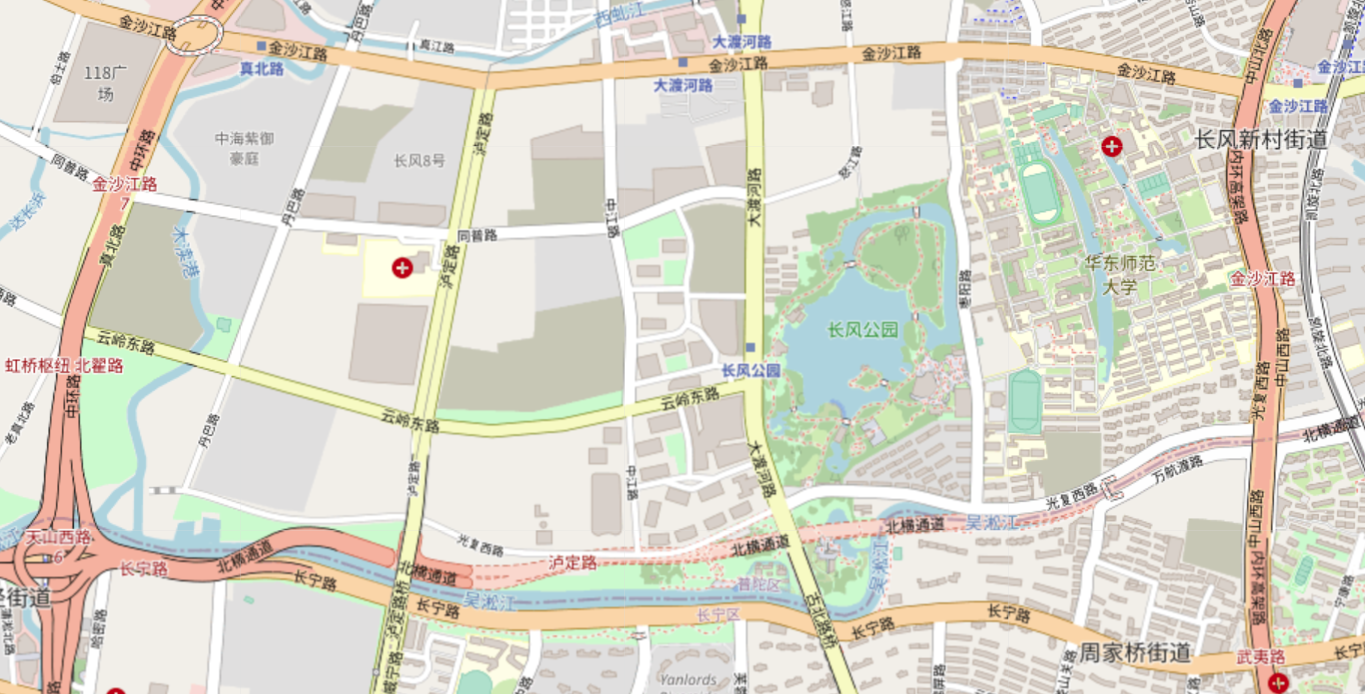
\includegraphics[width=\textwidth]{figures/real_road_network.png}
	\caption{上海市消防局附近的道路环境}
	\label{fig:real_road_network}
\end{figure}

\begin{figure}[H]
	\centering
	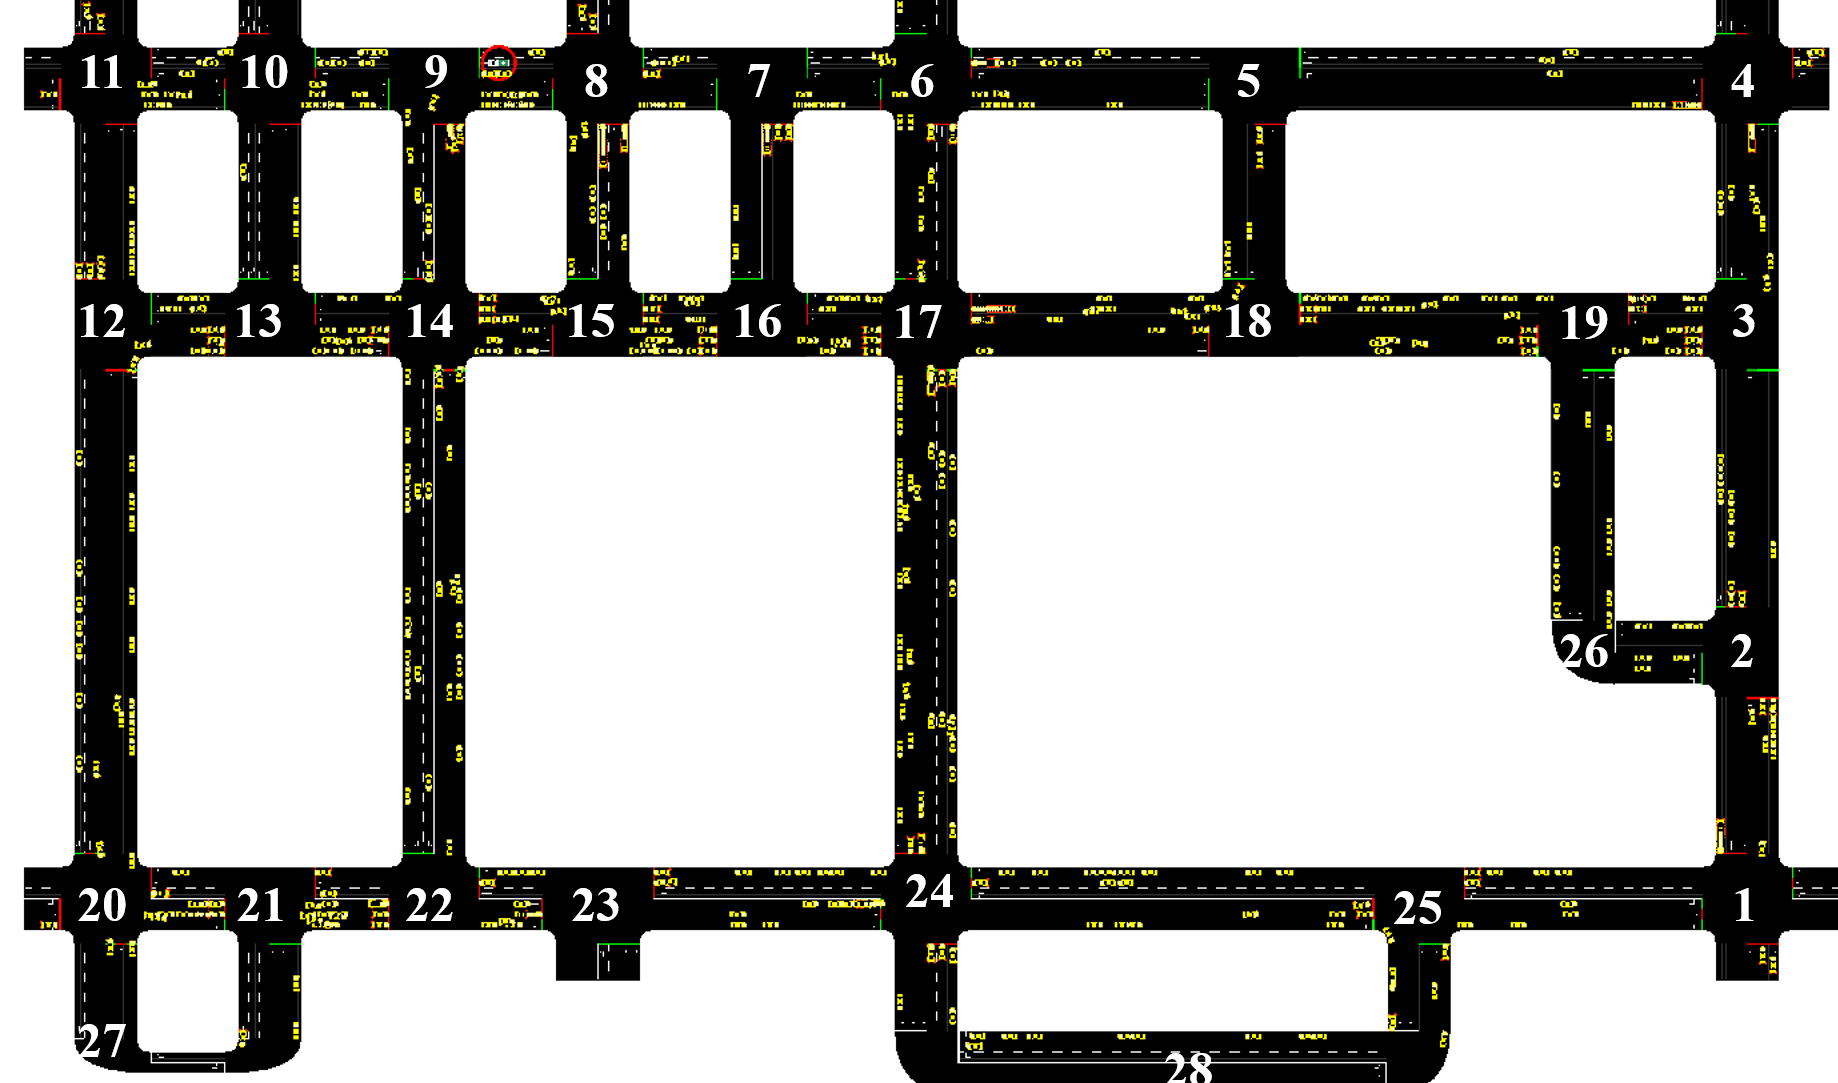
\includegraphics[width=\textwidth]{figures/road_network.png}
	\caption{交通路网}
	\label{fig:road_network}
\end{figure}

%为了证明本文方法的可用性以及有效性,将本文的信号控制方法与固定时长信号控制方法(the fixed-time control method,FTCM)、Min等人\cite{min}提出的FSPM方法(flexible signal preemption method,FSPM)以及Qin等人\cite{qin_control_2012}提出的侵入式抢占方法(intrusive signal preemption method,EVSP)相比较,固定时长信号控制方法保持信号相位时长不变。Min提出的弹性信号抢占方法是非侵入式抢占的代表。Qin等人提出的方法为侵入式抢占的代表。EV signal pre-emption (EVSP)

在同一路网条件下,对5辆应急车辆预先定义好不同的起止点,按照最短路径选定5条相应的应急车辆通行路线,路线编号分别为1、2、3、4、5,5条路线的路线距离以及路线如表\ref{table:route}所示,其中路线为应急车辆经过交叉口以及拐弯处的编号组成。各路线如图\ref{fig:route1}到图\ref{fig:route5}所示。

\begin{table}[H]
	\centering
	\caption{路线及其距离}
	\label{table:route}
	\begin{tabular}{|c|c|c|}
			\hline
			路线编号 & 路线距离(m) & 路线 \\
			\hline
			1 & 1256.59 & 1$\rightarrow$2$\rightarrow$3$\rightarrow$4$\rightarrow$5$\rightarrow$6$\rightarrow$7$\rightarrow$8$\rightarrow$9$\rightarrow$10$\rightarrow$11                \\ \hline
			2 & 9372.05 & 1$\rightarrow$2$\rightarrow$3$\rightarrow$4$\rightarrow$5$\rightarrow$6$\rightarrow$7$\rightarrow$8$\rightarrow$9$\rightarrow$10$\rightarrow$11$\rightarrow$12 \\ \hline
			3 & 8521.16 & 1$\rightarrow$2$\rightarrow$3$\rightarrow$4$\rightarrow$5$\rightarrow$6$\rightarrow$7$\rightarrow$8$\rightarrow$9$\rightarrow$14$\rightarrow$15                \\ \hline
			4 & 8465.14 & 11$\rightarrow$10$\rightarrow$9$\rightarrow$8$\rightarrow$7$\rightarrow$6$\rightarrow$5$\rightarrow$4$\rightarrow$3$\rightarrow$2$\rightarrow$1                \\ \hline
			5 & 5938.61 & 20$\rightarrow$27$\rightarrow$21$\rightarrow$22$\rightarrow$14$\rightarrow$9$\rightarrow$8$\rightarrow$7$\rightarrow$6 \\ \hline
	\end{tabular}
\end{table}

\begin{figure}[H]
	\centering
	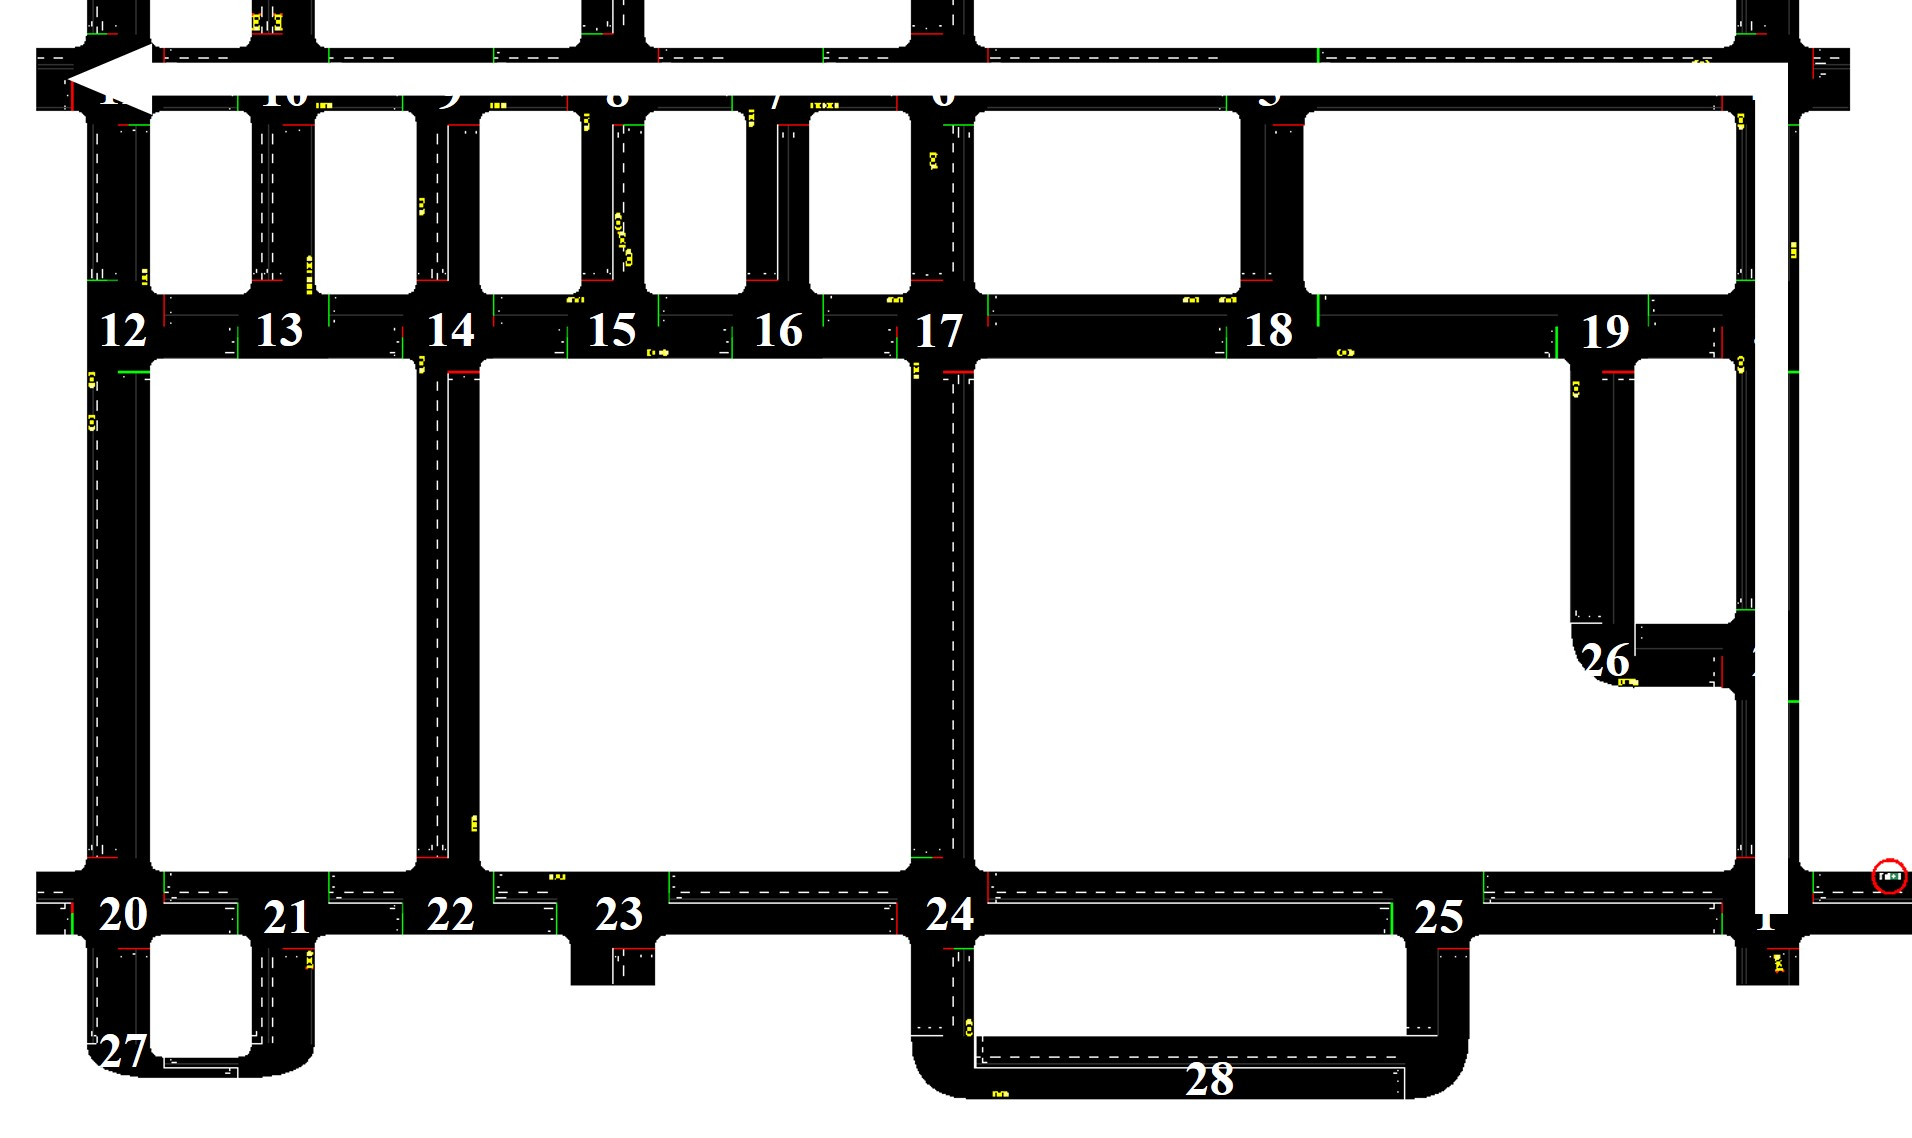
\includegraphics[width=\linewidth]{figures/route1.jpg}
	\caption{路线1}
	\label{fig:route1}
\end{figure}

\begin{figure}[H]
	\centering
	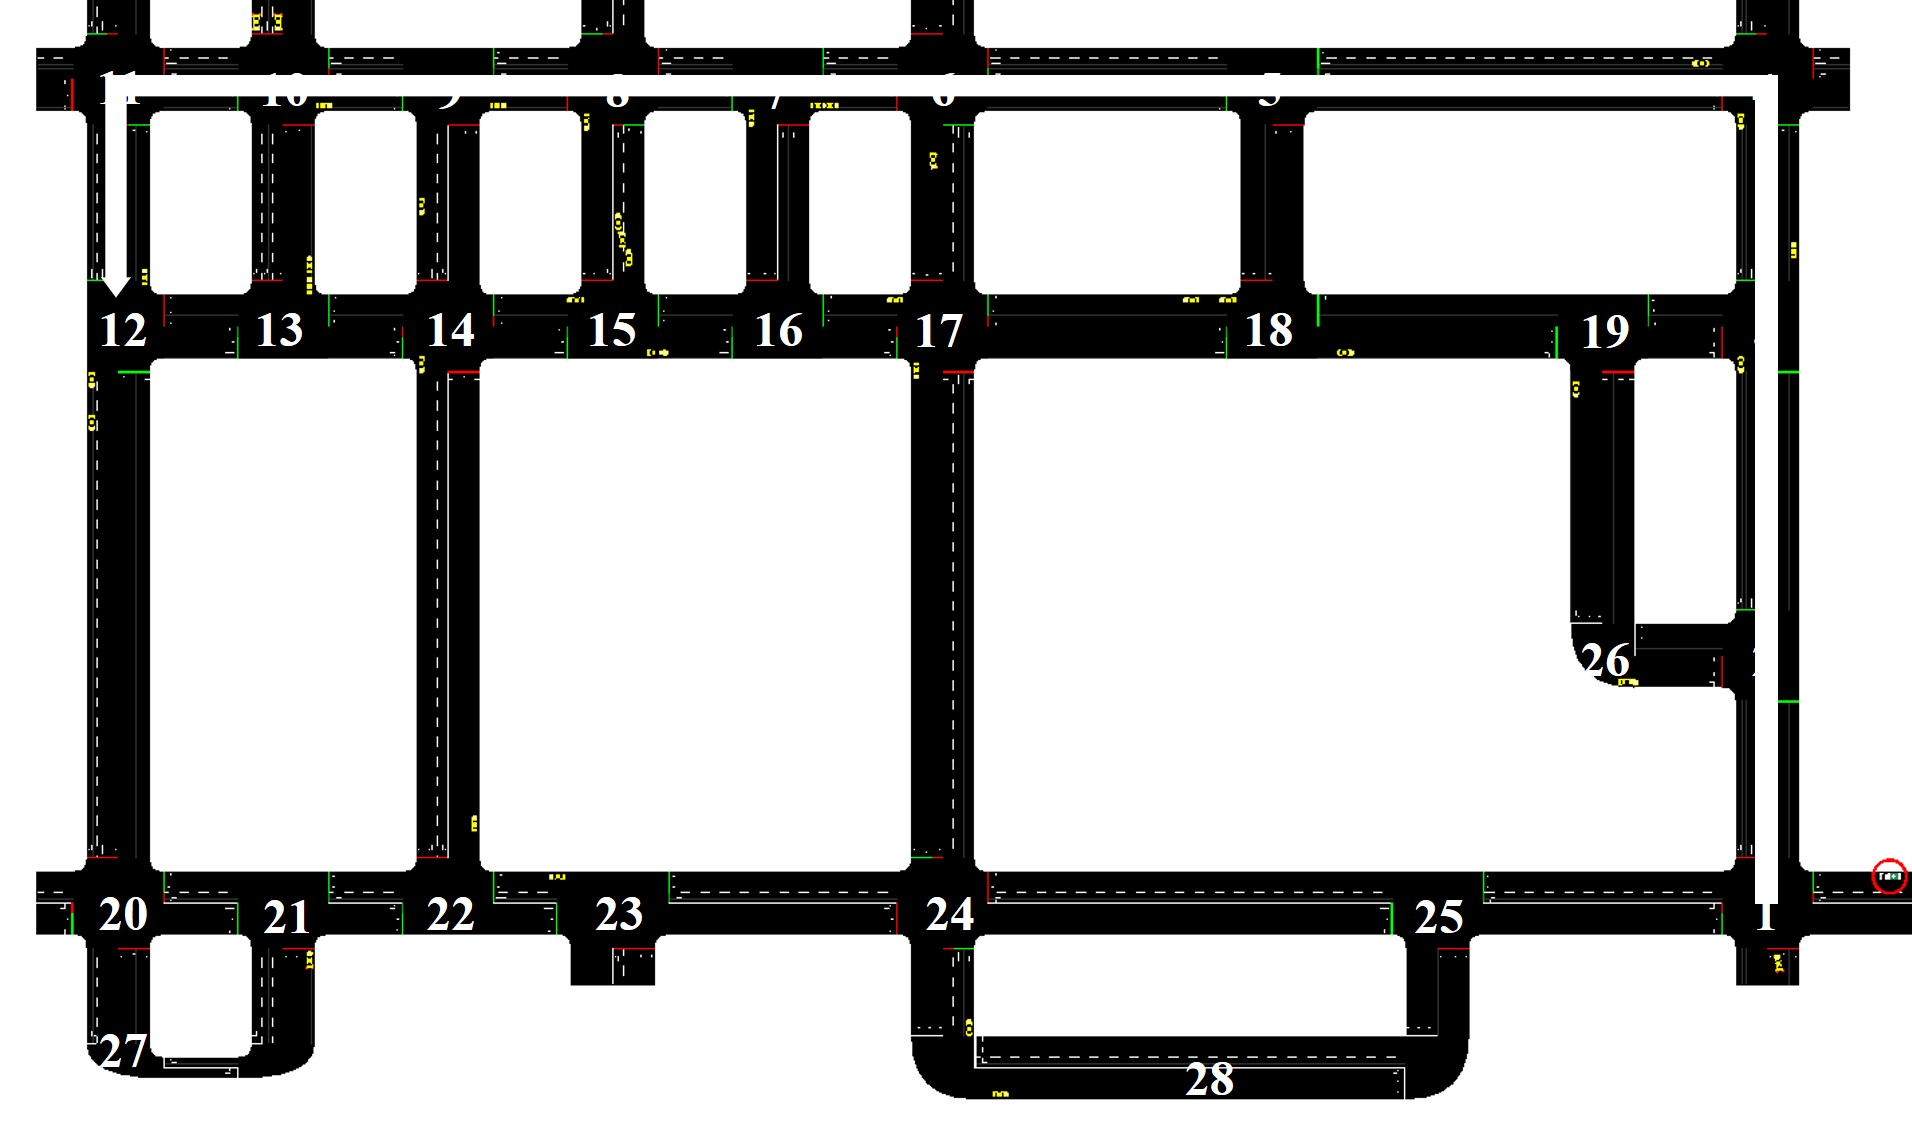
\includegraphics[width=\linewidth]{figures/route2.jpg}
	\caption{路线2}
	\label{fig:route2}
\end{figure}

\begin{figure}[H]
	\centering
	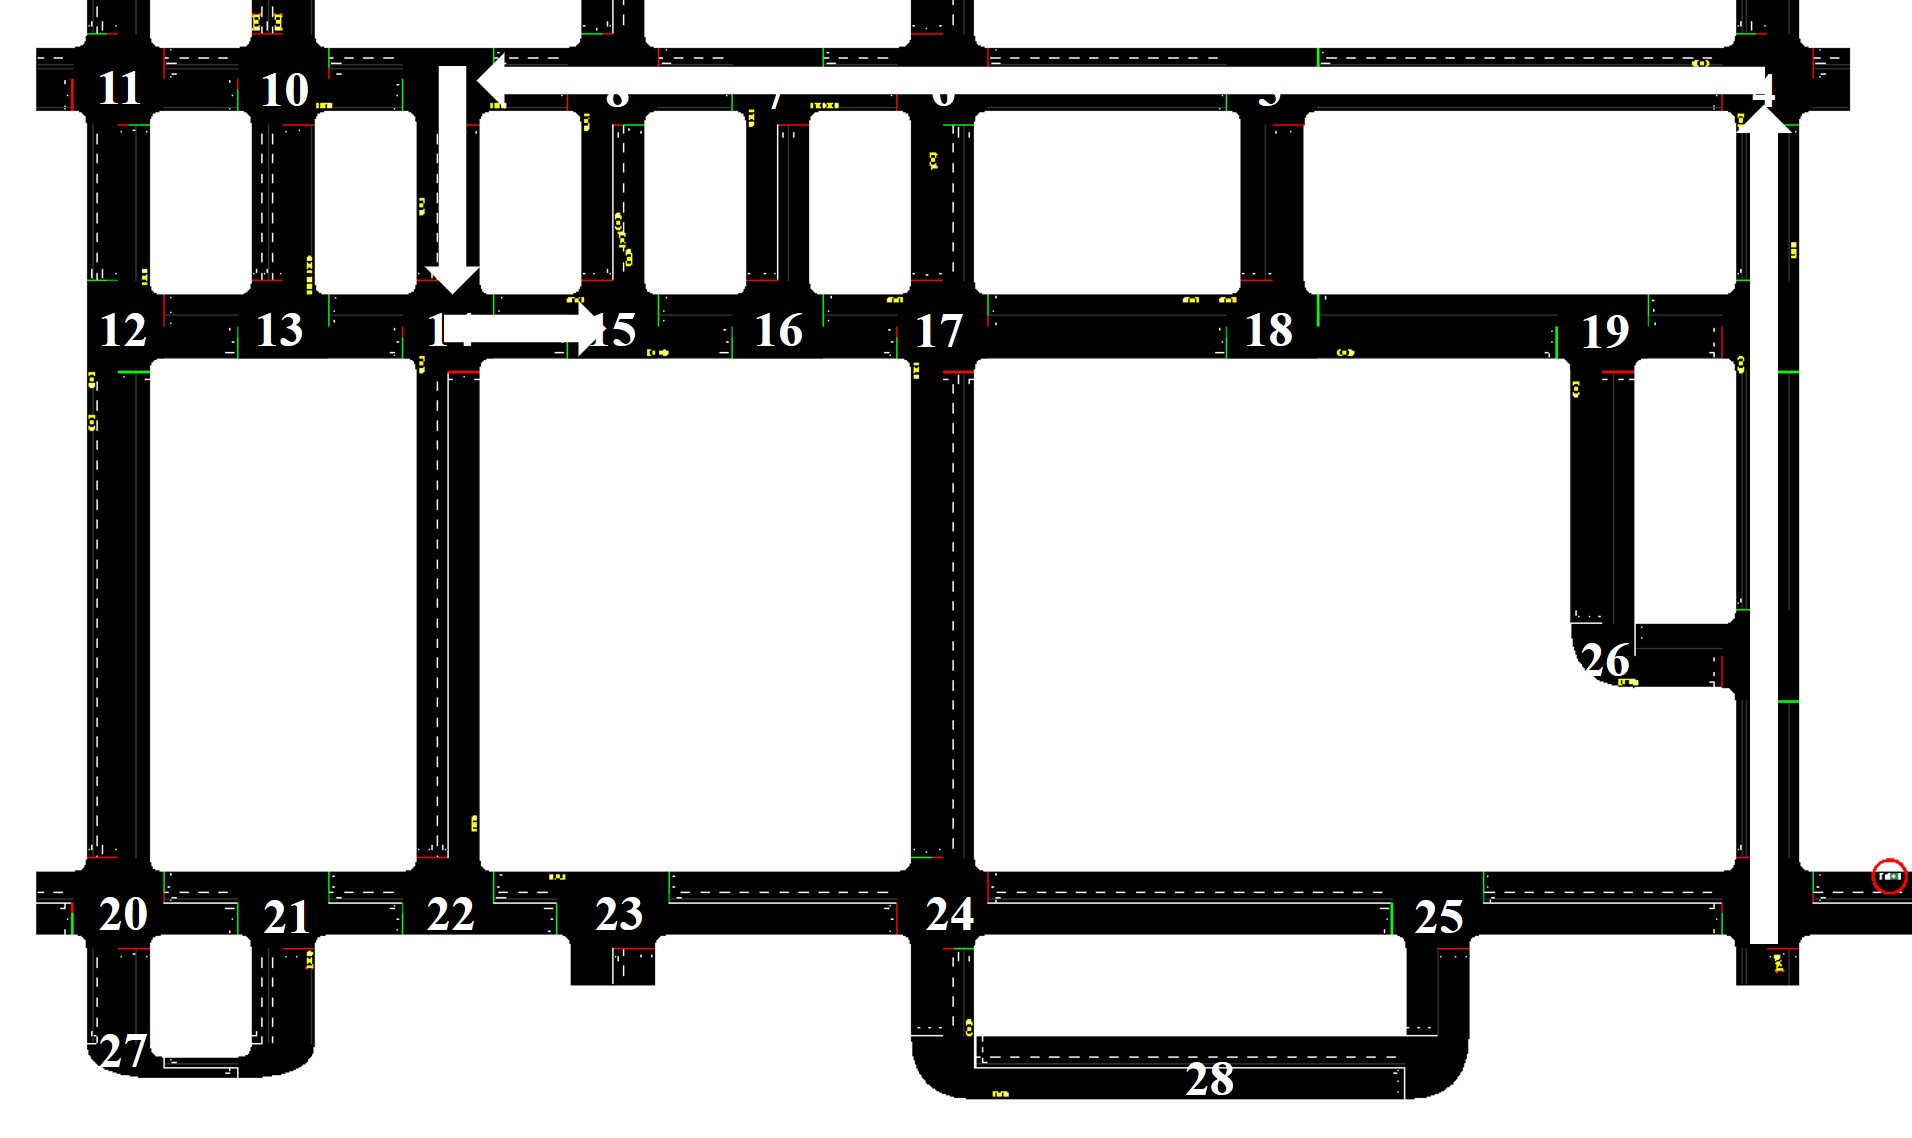
\includegraphics[width=\linewidth]{figures/route3.jpg}
	\caption{路线3}
	\label{fig:route3}
\end{figure}

\begin{figure}[H]
	\centering
	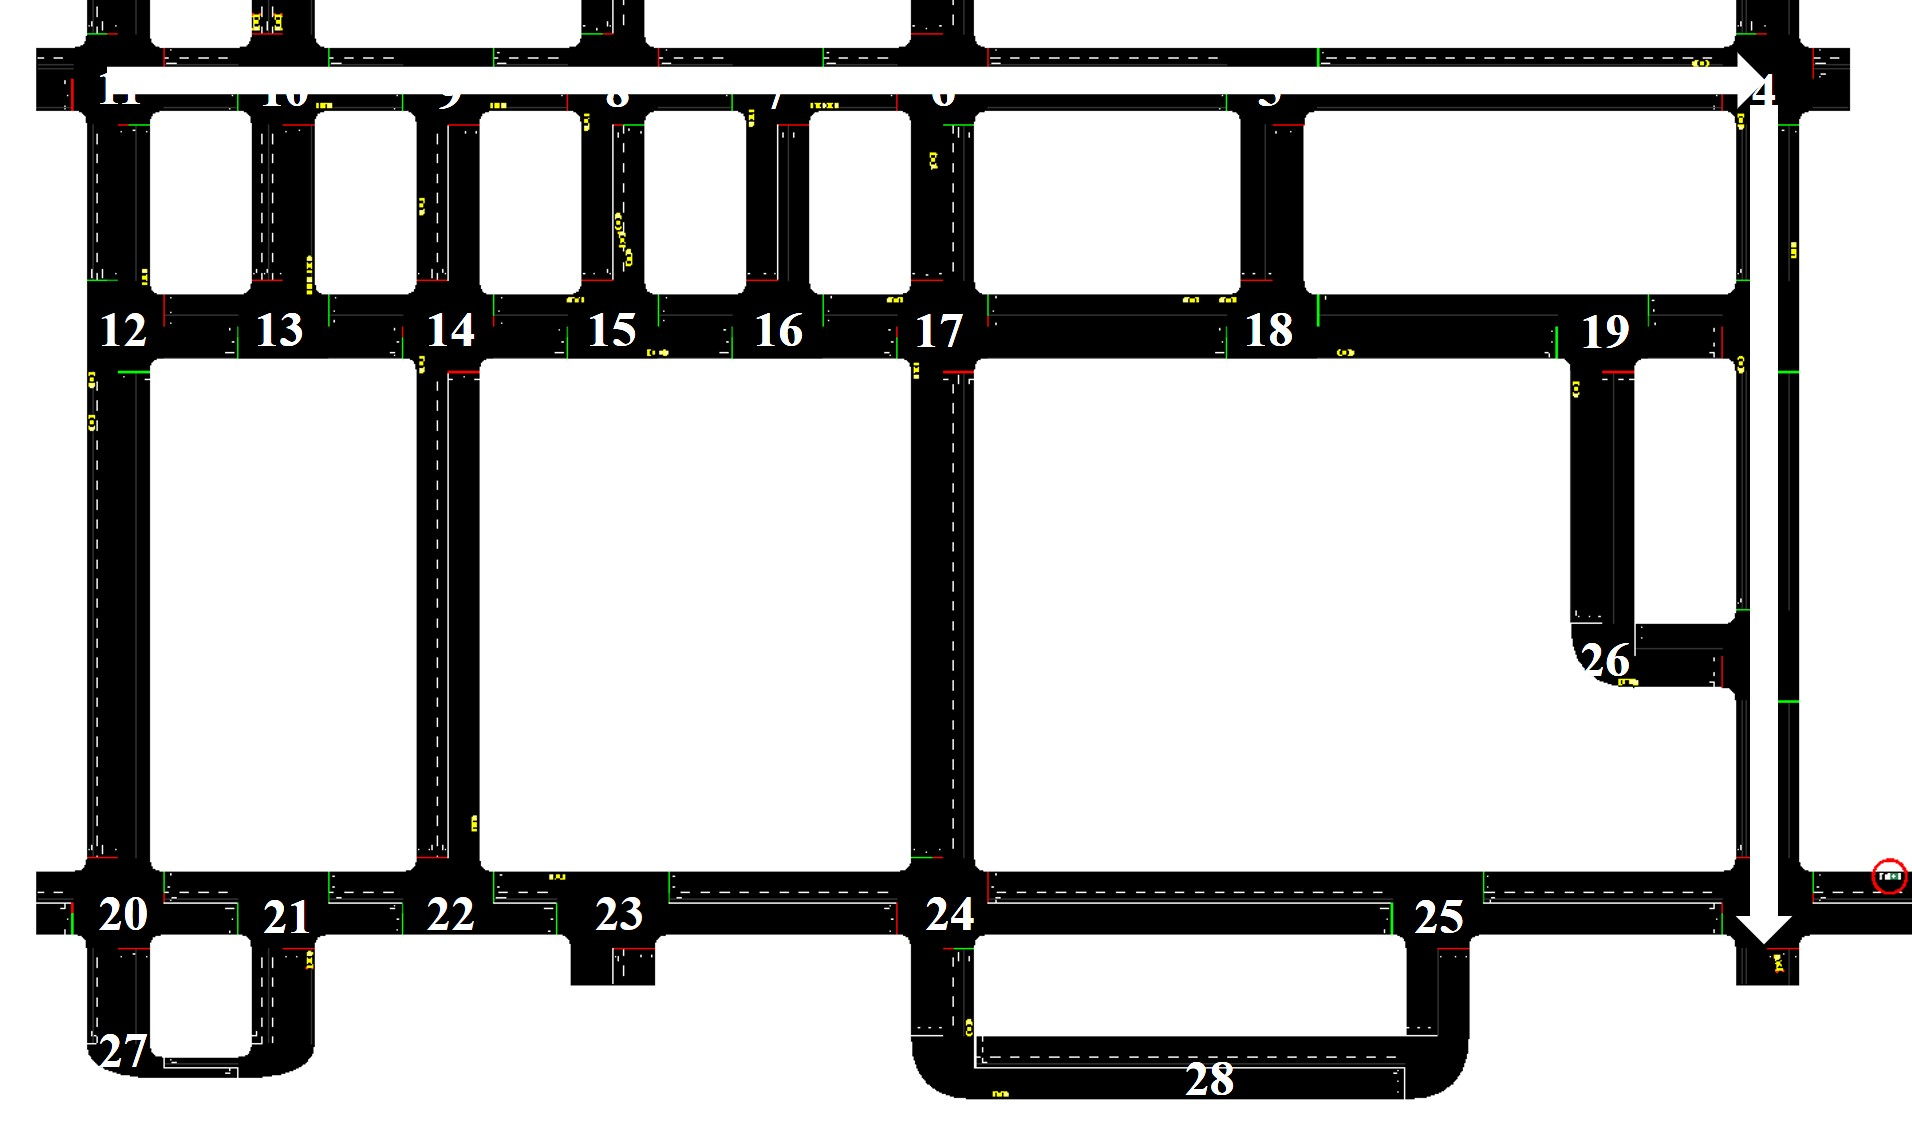
\includegraphics[width=\linewidth]{figures/route4.jpg}
	\caption{路线4}
	\label{fig:route4}
\end{figure}

\begin{figure}[H]
	\centering
	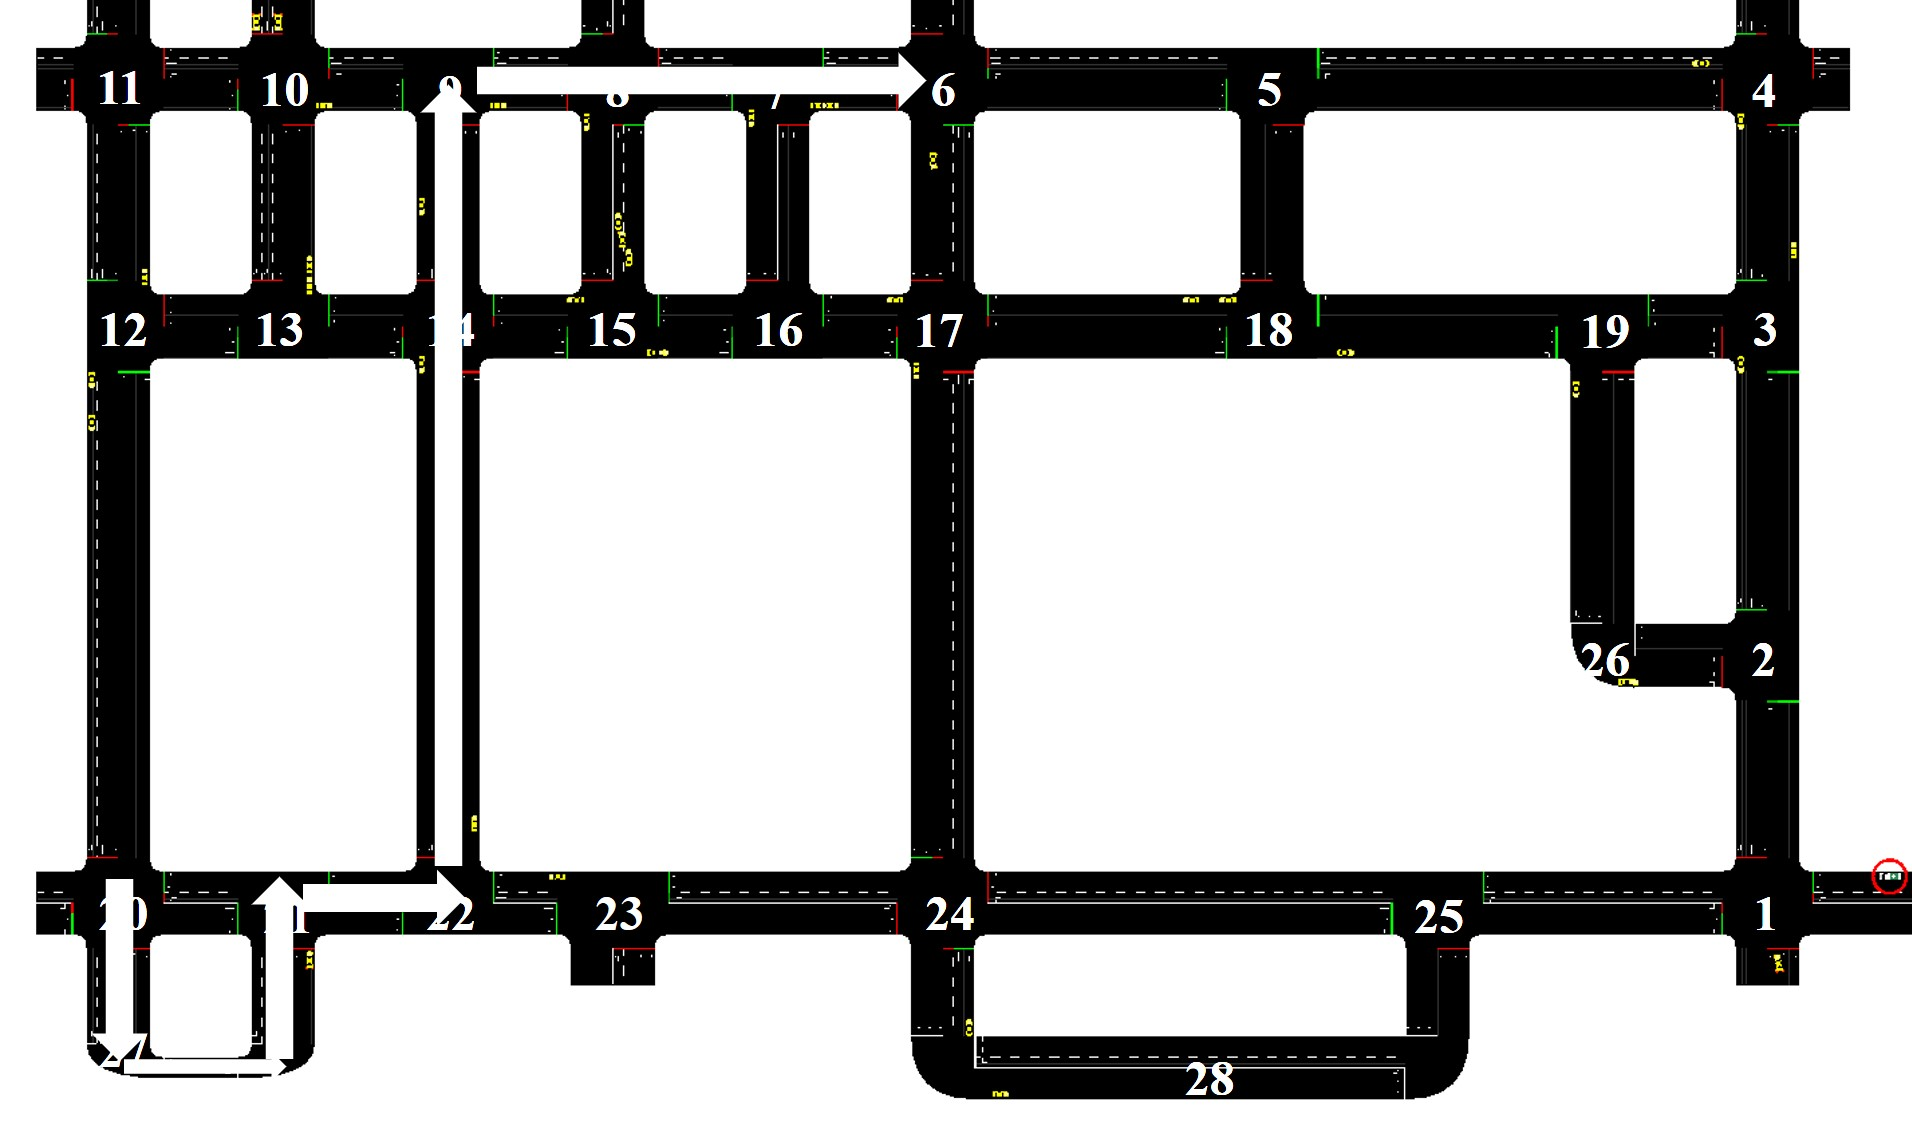
\includegraphics[width=\linewidth]{figures/route5.jpg}
	\caption{路线5}
	\label{fig:route5}
\end{figure}

通过SUMO设置不同交通规模产生不同的交通流量,通过设置交通规模能够按比例放大或缩小整个交通流量,本文设置了4种不同的交通规模,分别为1、2、3和4,表示为道路畅通、道路较为拥堵、道路中度拥堵以及道路严重拥堵,分别代表在原本交通流量的基础上,交通流量按比例扩大到1倍、2倍、3倍和4倍。对于交通规模为1的实验,路网中有2400辆普通车辆,因此本文一共对48万条汽车数据进行了处理。

为了回答实验目的中的第一个问题,将本文方法与固定时长信号控制方法(the fixed-time control method,FTCM)进行对比,应急车辆的速度偏差越小,表明应急车辆行驶更平稳,也就代表了应急车辆在行驶的过程中,前方普通车辆对应急车辆的阻碍较小,因此表明普通车辆为应急车辆让行了。本文方法是在固定时长信号控制方法的基础上进行信号控制的,因此固定时长信号控制方法可作为对照组,比较使用本文方法和不使用本文方法的区别。5辆应急车辆对应5条行驶路线,交通规模分为道路畅通、道路较为拥堵、道路中度拥堵以及道路严重拥堵。本文使用本文方法和FTCM在交通规模分别为道路畅通、道路较为拥堵、道路中度拥堵以及道路严重拥堵的环境下进行多次实验,对应急车辆的速度偏差进行对比分析。

%本文在图\ref{fig:road_network}的路网条件下,对5辆应急车辆预先定义好不同的起止点,按照最短路径选定5条相应的应急车辆通行路线,路线编号分别为1、2、3、4、5,5条路线的路线距离以及路线如表\ref{table:route}所示,其中路线为应急车辆经过交叉口以及拐弯处的编号组成。通过SUMO设置不同交通规模产生不同的交通流量,通过设置交通规模能够按比例放大或缩小整个交通流量,本文设置了4种不同的交通规模,分别为1、2、3和4,表示为道路畅通、道路较为拥堵、道路中度拥堵以及道路严重拥堵,分别代表在原本交通流量的基础上,交通流量按比例扩大到1倍、2倍、3倍和4倍。对于交通规模为1的实验,路网中有2400辆普通车辆,因此本实验一共对48万条汽车数据进行了处理。

为了回答实验目的中的第二个问题,将本文的信号控制方法与固定时长信号控制方法(fixed-time control method,简称FTCM)、Min等人\cite{min}提出的弹性信号抢占方法(flexible signal preemption  method,简称FSPM)以及Qin等人\cite{qin_control_2012}提出的应急车辆信号抢占方法(emergency vehicle signal pre-emption,简称EVSP)相比较。固定时长信号控制方法保持信号相位时长不变。Min提出的弹性信号抢占方法是非侵入式抢占的代表。Qin等人提出的方法为侵入式抢占的代表。与实验一类似,5辆应急车辆对应5条行驶路线,交通规模分为道路畅通、道路较为拥堵、道路中度拥堵以及道路严重拥堵。本文使用本文方法、FTCM、FSPM和EVSP在交通规模分别为道路畅通、道路较为拥堵、道路中度拥堵以及道路严重拥堵的环境下进行多次实验,对应急车辆的旅行时间进行对比分析。

为了回答实验目的中的第三个问题,将本文方法与固定时长信号控制方法进行对比。本文使用平均等待时间来反映应急车辆优先通行对整个路网的影响。如果本文方法平均等待时间小于或等于固定时长信号控制方法的平均等待时间,则表明本文方法不会对整个路网造成明显影响。5辆应急车辆对应5条行驶路线,交通规模分为道路畅通、道路较为拥堵、道路中度拥堵以及道路严重拥堵。使用本文方法和FTCM在交通规模分别为道路畅通、道路较为拥堵、道路中度拥堵以及道路严重拥堵的环境下进行多次实验,对应急车辆的平均等待时间进行对比分析。

%与实验一类似,五辆应急车辆对应五条行驶路线,交通规模分为道路畅通、道路较为拥堵、道路中度拥堵以及道路严重拥堵。我们对整个交通路网中所有车辆的平均等待时间进行分析统计。

\section{实验环境及参数设置}
实验环境配置如表\ref{table:shiyanhuanjing}所示,实验使用的CPU型号为Intel(R) Core(TM) i7-10710U,操作系统为Windows 10,内存为16GB,使用的仿真平台为SUMO 1.8.0,Python版本为3.8。实验参数设置如表\ref{table:shiyancanshu}所示,其中${\beta}$值为0.5,经过多次重复实验,发现${\beta}$的值对实验结果影响不明显,其值主要取决于应用场景,因此本文使得其值为0.5,与文献\cite{min}保持一致。


%实验使用的CPU型号为Intel(R) Core(TM) i7-10710U,操作系统为Windows 10,内存为16GB,使用的仿真平台为SUMO 1.8.0,Python版本为3.8。实验参数设置如表\ref{table:shiyancanshu}所示。其中${\beta}$值为0.5,经过多次重复实验,发现${\beta}$的值对实验结果影响不明显,其值主要取决于应用场景,因此本文使得其值为0.5,与文献\cite{min}保持一致。

%车辆启动损失时间${T_{lost}}$为5s,十字路口安全时间间隔${SIT}$为5s,T型路口安全时间间隔${SIT}$为3s,交叉口普通车辆为应急车辆让行所需时间${YT}$为5s,相位最短路灯时间为${\tau_i^{min}}$为7s,相位最长时间${\tau_i^{max}}$为200s,平均排队车辆数${AVE_i^k}$为5辆,经过多次重复实验,本文发现${\beta}$的值对实验结果影响不明显,其值主要取决于应用场景,本文使得其值为0.5。

\begin{table}[H]
	\centering
	\caption{实验环境配置}
	\label{table:shiyanhuanjing}
	\begin{tabular}{|c|c|}
		\hline
		CPU & Intel(R) Core(TM) i7-10710U \\ \hline
		操作系统 & Windows 10 \\ \hline
		内存 & 16GB \\ \hline
		Python版本 & 3.8 \\ \hline
		SUMO版本 & 1.8.0 \\ \hline
	\end{tabular}
\end{table}

\begin{table}[H]
	\centering
	\caption{实验参数配置}
	\label{table:shiyancanshu}
	\begin{tabular}{|c|l|}
		\hline
		参数 & 值 \\ \hline
		${\beta}$ & 0.5 \\ \hline
		${T_i}$ & 对于十字路口,${T_i}$为200s,对于T型路口${T_i}$为90s \\ \hline
		${PN}$ &  对于十字路口,${T_i}$为4,对于T型路口${T_i}$为2 \\ \hline
		${g_i^k}$ & 对于十字路口,${T_i}$为45s,对于T型路口${T_i}$为42s  \\ \hline
		${T_{lost}}$ & 5s \\ \hline
		${SIT}$ & 5s \\ \hline
		${YR}$ & 对于十字路口,${T_i}$为5s,对于T型路口${T_i}$为3s \\ \hline
		${YT}$ & 5s \\ \hline
		${\tau_i^{min}}$ & 7s \\ \hline
		${\tau_i^{max}}$ & 200s \\ \hline
		${T_i^{min}}$ & 对于十字路口,${T_i}$为60s,对于T型路口${T_i}$为20s \\ \hline
		${T_i^{max}}$ & 对于十字路口,${T_i}$为820s,对于T型路口${T_i}$为406s \\ \hline
		${G_{minS}}$ & 7s  \\ \hline
		${AVE_i^k}$ & 5辆 \\ \hline
	\end{tabular}
\end{table}

此外,实验中使用解决凸优化问题的Python嵌入式建模语言CVXPY实现二次规划算法和线性规划算法\cite{diamond2016cvxpy, agrawal2018rewriting}。在实验中,二次规划算法与线性规划算法均能够在1秒时间内返回结果,因此在一定程度上保障了本文方法的实时性。在实际生活中,二次规划算法和线性规划算法已经得到了广泛的应用,根据弹性信号抢占方法\cite{min}中实地实验结果表明,现实生活中,二次规划在非侵入式抢占时表现良好。

%但是由于二次规划算法受到约束条件的限制,运算需要一定的时间,这与约束条件有关,但是在本文的实验中,二次规划算法能够在几秒时间内返回结果。我本使用python的CVXPY库中的solver的qp和lp方法分别实现二次规划方法和线性规划方法。

%二次规划能够在0.362s之内完成计算

%CVXPY是一种用于凸优化问题的python嵌入式建模语言。它自动将问题转换成标准形式,调用求解器,并解包结果。


\section{实验结果分析}
\subsection{应急车辆速度平稳性分析}
本文使用应急车辆的速度标准差来反应应急车辆从起点到终点行驶过程中速度的浮动程度,应急车辆速度标准差的计算方式如下所示:
\begin{equation}
	\label{equation:sigma}
	\sigma = \dfrac{\sqrt{\sum_{t_0}^{t_n} (v-\bar{v})^2 dt}}{t_n}
\end{equation}
${\sigma}$为实时速度标准差,其值为应急车辆从出发时刻${t_0}$到应急车辆到达目的地时刻${t_n}$期间实时速度${v}$的标准差,反映了应急车辆在行驶的过程中停车与慢速行驶的频率,标准差越小,反映了应急车辆的行驶速度越稳定。

本文测试了应急车辆在不同交通规模下,应急车辆的速度标准差在本文方法与固定时长信号控制方法(FTCM)的对比。为了使实验效果更加明显,首先假设应急车辆的应急救援等级为特别重大(I级),即应急车辆执行的任务。然后对5辆应急车辆分别在道路畅通、道路较为拥堵、道路中度拥堵以及道路严重拥堵四种交通规模下进行实验,对应急车辆的速度偏差进行对比分析。

%图\ref{fig:std_smooth}、\ref{fig:std_relatively}、\ref{fig:std_moderate}、\ref{fig:std_severely}分别对应5辆应急车辆在道路畅通、道路较为拥堵、道路中度拥堵以及道路严重拥堵的旅行时间,从图中可以看出,使用本文方法能够明显提升应急车辆在行驶过程中速度的稳定性,本文的信号控制方法能够使得应急车辆以更快且更稳定的速度行驶。实验表明本文降低道路饱和度的方法使应急车辆保持高匀速行驶优势明显。

图\ref{fig:std_smooth}、\ref{fig:std_relatively}、\ref{fig:std_moderate}、\ref{fig:std_severely}分别对应5辆应急车辆在道路畅通、道路较为拥堵、道路中度拥堵以及道路严重拥堵的旅行时间,从图中可以看出,使用本文方法能够明显提升应急车辆在行驶过程中速度的稳定性,本文的信号控制方法能够使得应急车辆以更快且更稳定的速度行驶。实验表明本文方法使应急车辆保持高匀速行驶优势明显。

%如图\ref{fig:std_smooth}所示,应急车辆在道路畅通的情况下,使用本文方法能够明显提升应急车辆在行驶过程中速度的稳定性,应急车辆能够以更平稳的速度行驶。

\begin{figure}[H]
	\centering
	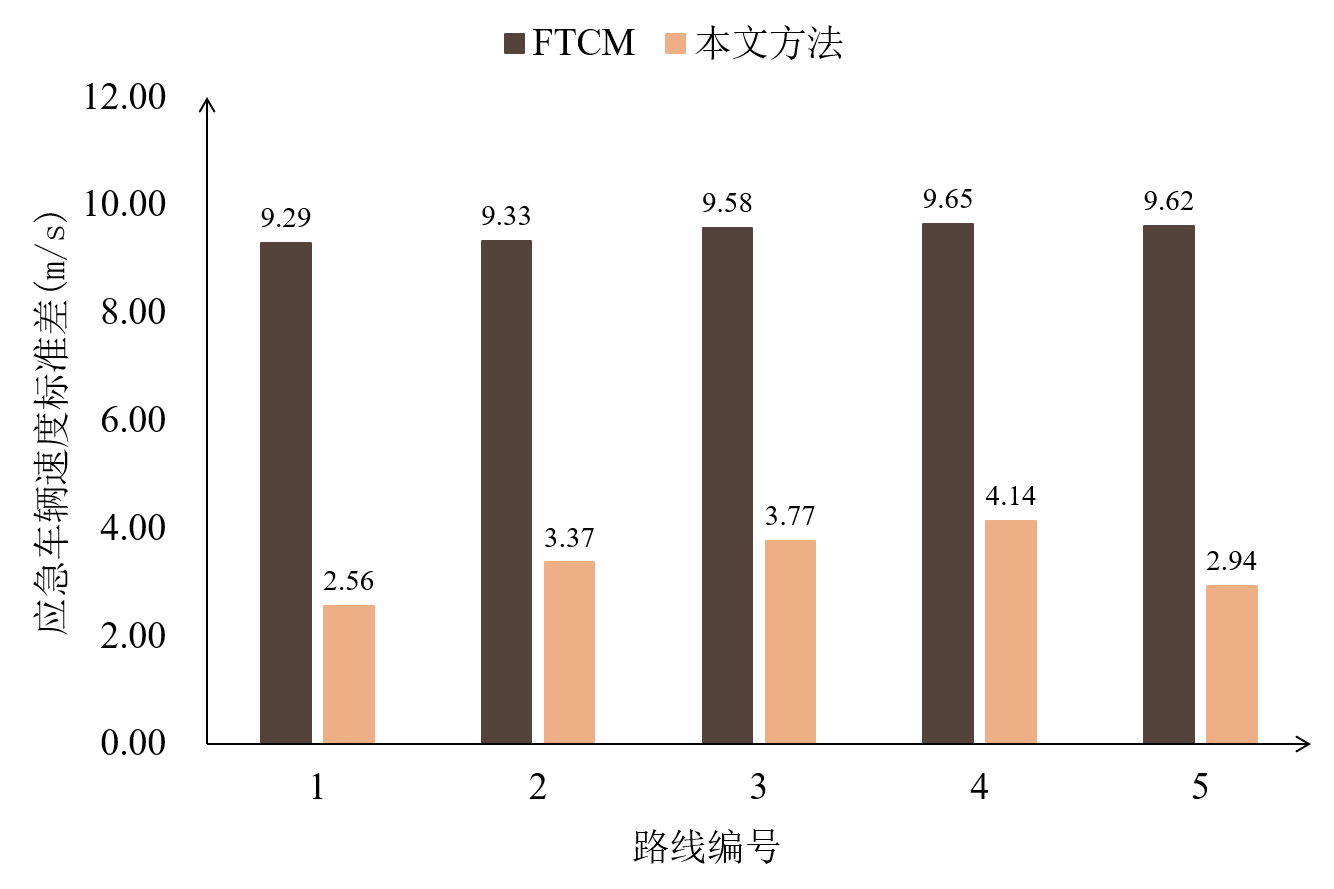
\includegraphics[width=\linewidth]{figures/std_smooth.png}
	\caption{道路畅通时速度标准差结果对比图}
	\label{fig:std_smooth}
\end{figure}

%如图\ref{fig:std_relatively}所示,应急车辆在道路相对拥堵的情况下,使用本文方法能够明显提升应急车辆在行驶过程中速度的稳定性,应急车辆能够以更平稳的速度行驶。
\begin{figure}[H]
	\centering
	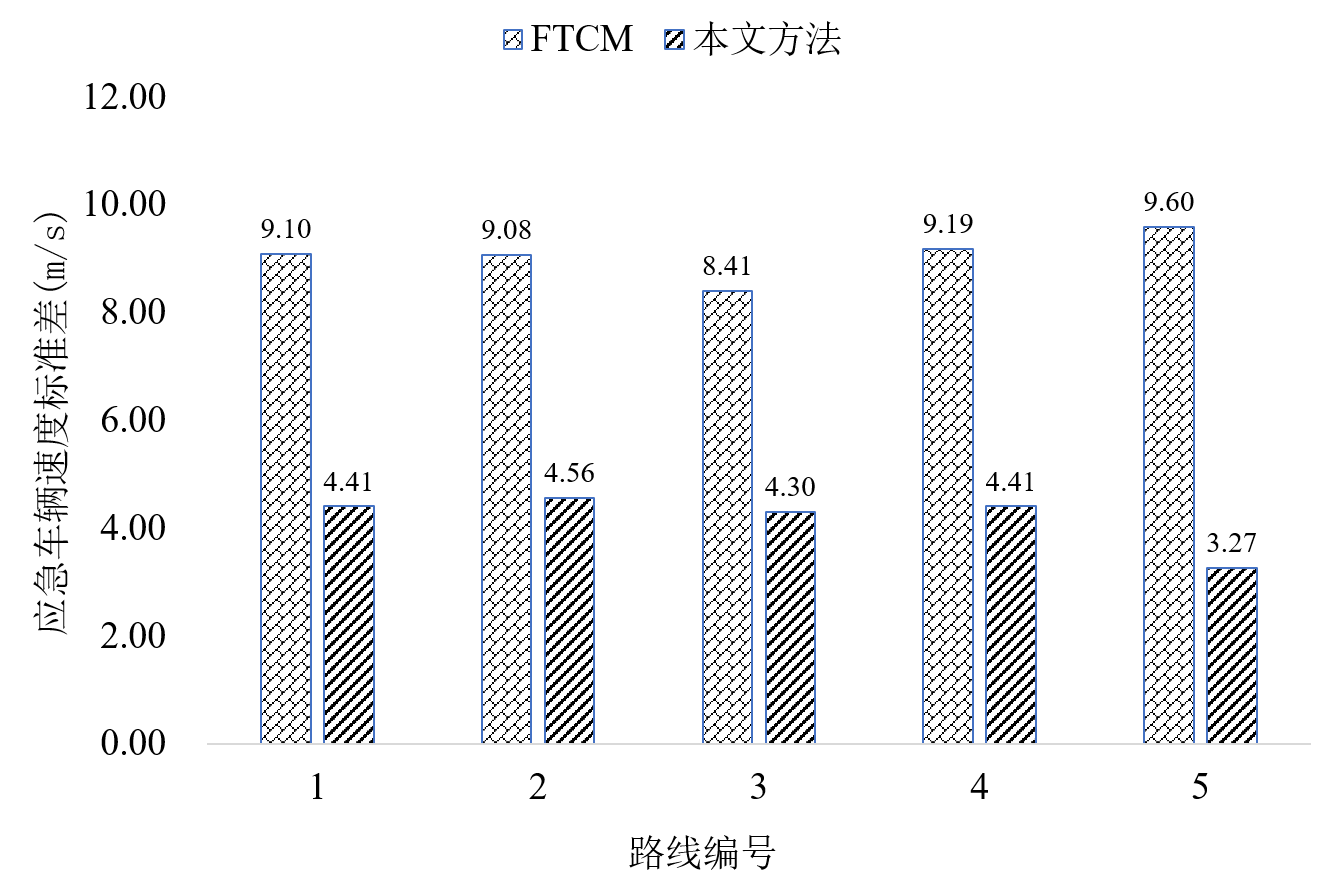
\includegraphics[width=\linewidth]{figures/std_relatively.png}
	\caption{道路相对拥堵时速度标准差结果对比图}
	\label{fig:std_relatively}
\end{figure}

%如图\ref{fig:std_moderate}所示,应急车辆在道路中度拥堵的情况下,使用本文方法能够明显提升应急车辆在行驶过程中速度的稳定性,应急车辆能够以更平稳的速度行驶。

\begin{figure}[H]
	\centering
	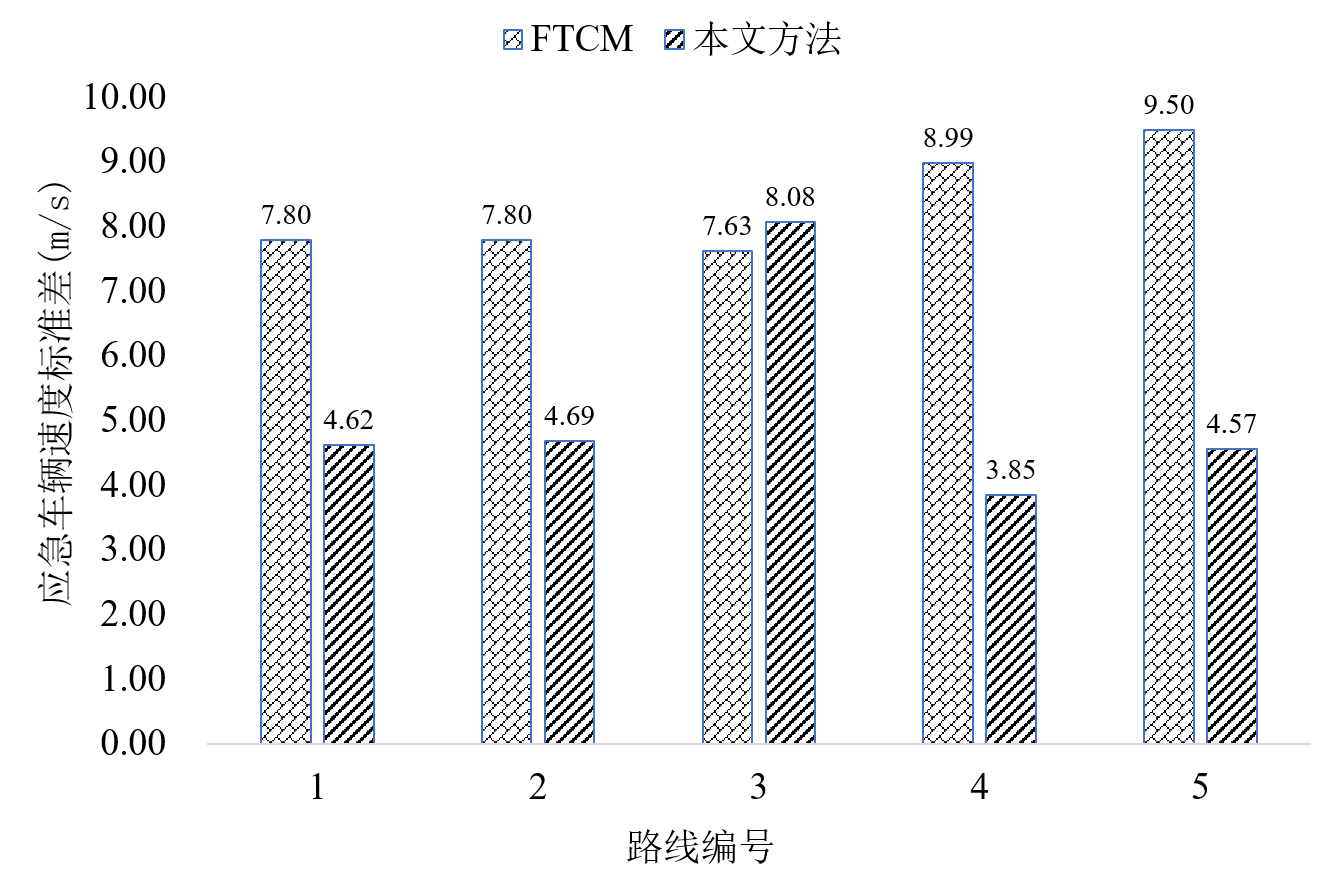
\includegraphics[width=\linewidth]{figures/std_moderate.png}
	\caption{道路中度拥堵时速度标准差结果对比图}
	\label{fig:std_moderate}
\end{figure}

%如图\ref{fig:std_moderate}所示,应急车辆在道路中度拥堵的情况下,使用本文方法能够相对提升应急车辆在行驶过程中速度的稳定性,应急车辆能够以更平稳的速度行驶。

\begin{figure}[H]
	\centering
	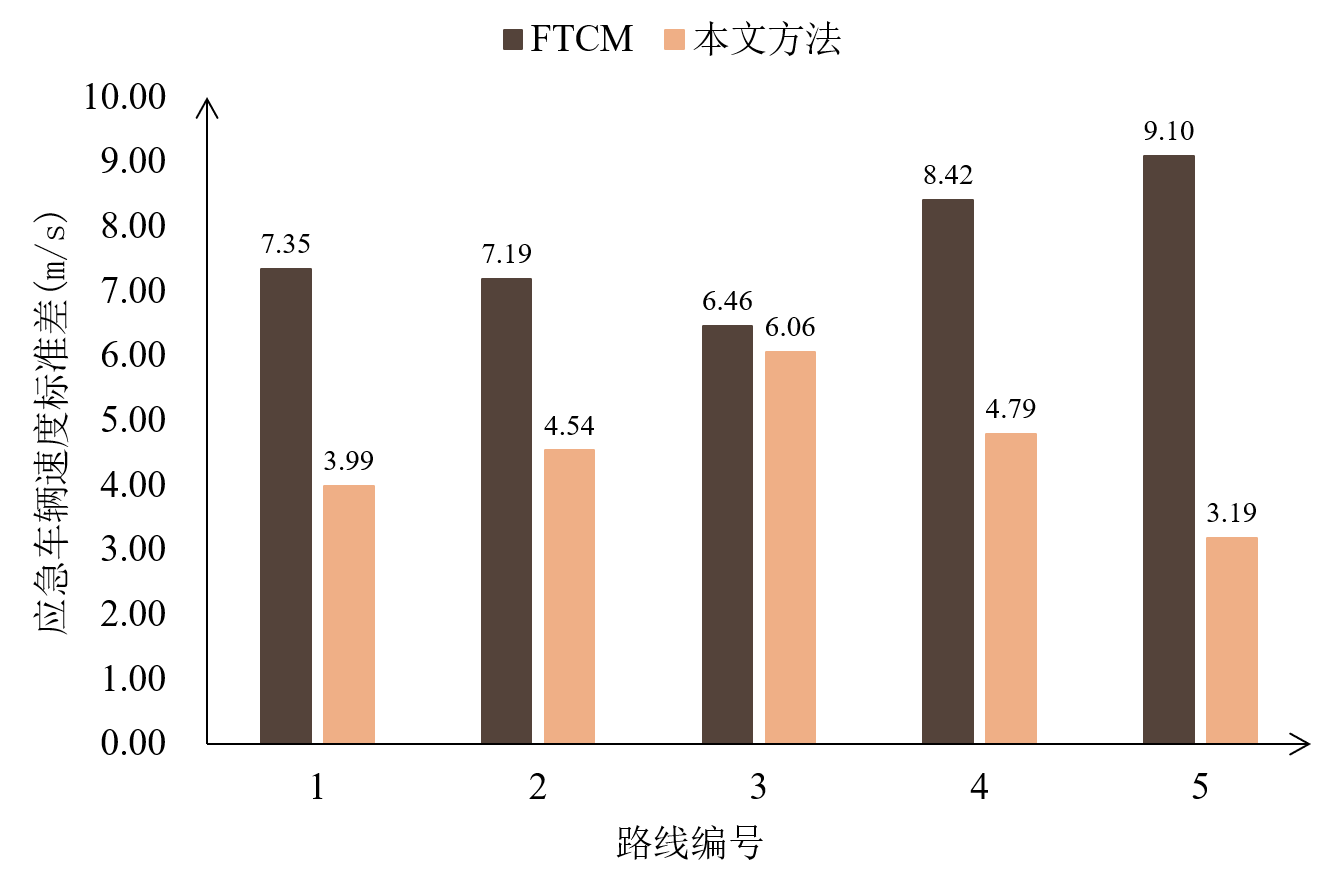
\includegraphics[width=\linewidth]{figures/std_severely.png}
	\caption{道路严重拥堵时速度标准差结果对比图}
	\label{fig:std_severely}
\end{figure}

\subsection{应急车辆旅行时间分析}
本文测试了应急车辆在不同交通拥堵情况下,应急车辆的旅行时间在本文方法与FTCM、FSPM以及EVSP对比。首先假设应急车辆的应急救援等级为特别重大(I级),即应急车辆执行的任务非常紧急,然后让5辆应急车辆分别在道路畅通、道路较为拥堵、道路中度拥堵以及道路严重拥堵四种交通规模下进行反复多次实验。

如图\ref{fig:travel_time_smooth}表示在道路畅通情况下,5辆应急车辆分别采用FTCM、FSPM、EVSP以及本文方法在路线1至5上的旅行时间。图中横坐标为5辆应急车辆的路线编号,纵坐标为应急车辆的旅行时间。由图可知,本文方法相比于其他三种方法,具有明显优势。图\ref{fig:travel_time_relatively_congestion}表示在道路较为拥堵情况下,5辆应急车辆分别采用FTCM、FSPM、EVSP以及本文方法在路线1至5上的旅行时间。图片表明,本文方法相比于其他三种方法,在道路较为拥堵的情况下仍然具有明显优势。图\ref{fig:travel_time_moderate_congestion}表示在道路中度拥堵情况下,5辆应急车辆分别采用FTCM、FSPM、EVSP以及本文方法在路线1至5上的旅行时间。图片表明,本文方法相比于其他三种方法,在道路中度拥堵的情况下仍然具有明显优势。图\ref{fig:travel_time_severe_congestion}表示在道路严重拥堵情况下,5辆应急车辆分别采用FTCM、FSPM、EVSP以及本文方法在路线1至5上的旅行时间。图片表明,本文方法相比于其他三种方法,在道路严重拥堵的情况下仍然具有明显优势。由此可知,绝大部分情况下本文方法能够有效缩短应急车辆的旅行时间,并且效果非常明显。即使在发生车祸的路段,也能够大幅度缩短应急车辆的旅行时间。

\begin{figure}[H]
	\centering
	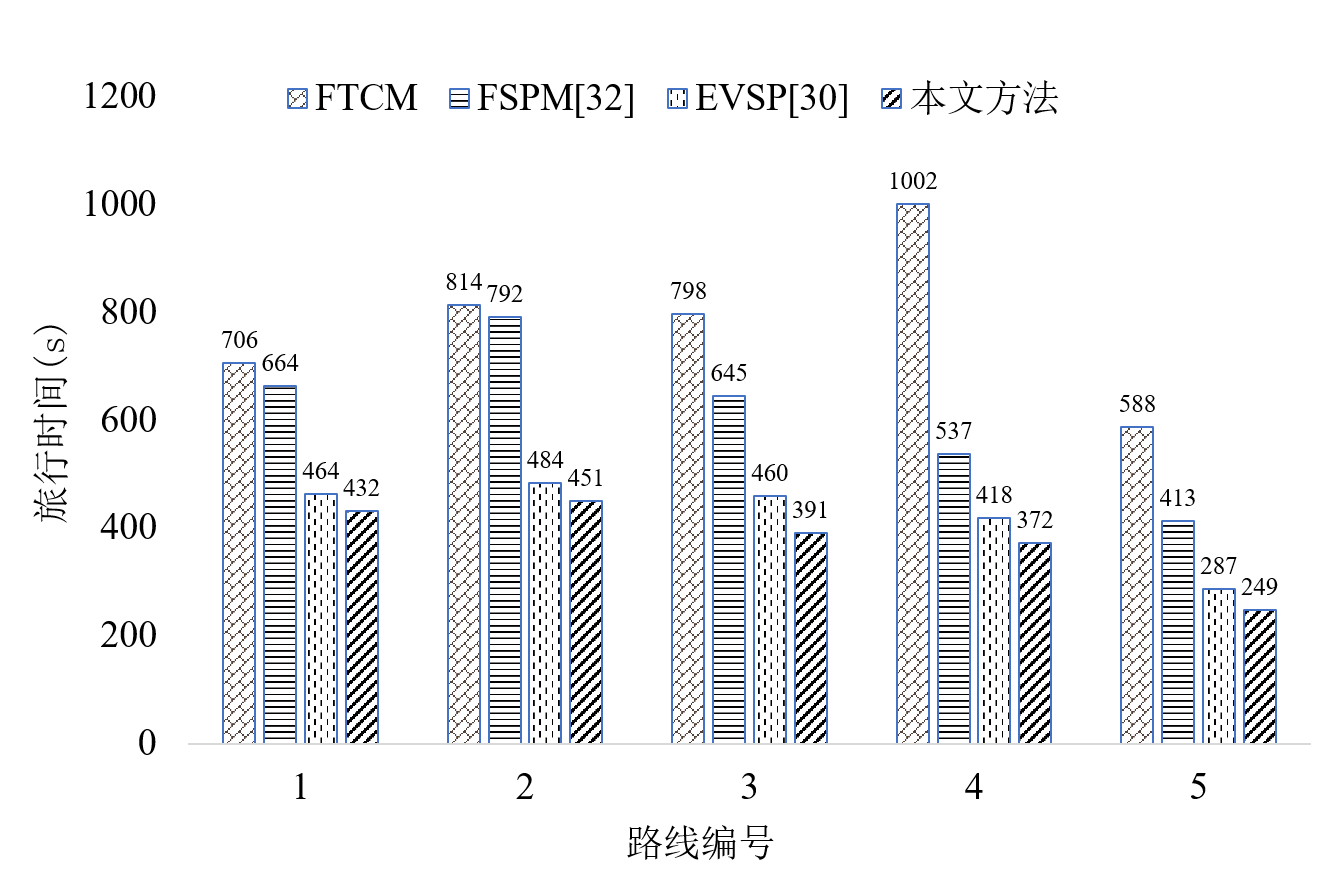
\includegraphics[width=\linewidth]{figures/travel_time1.png}
	\caption{道路畅通时旅行时间比较}
	\label{fig:travel_time_smooth}
\end{figure}

%图\ref{fig:travel_time_relatively_congestion}表示在道路较为拥堵情况下,5辆应急车辆分别采用FTCM、FSPM、EVSP以及本文方法在路线1至5上的旅行时间。图片表明,本文方法相比于其他三种方法,在道路较为拥堵的情况下仍然具有明显优势。

\begin{figure}[H]
	\centering
	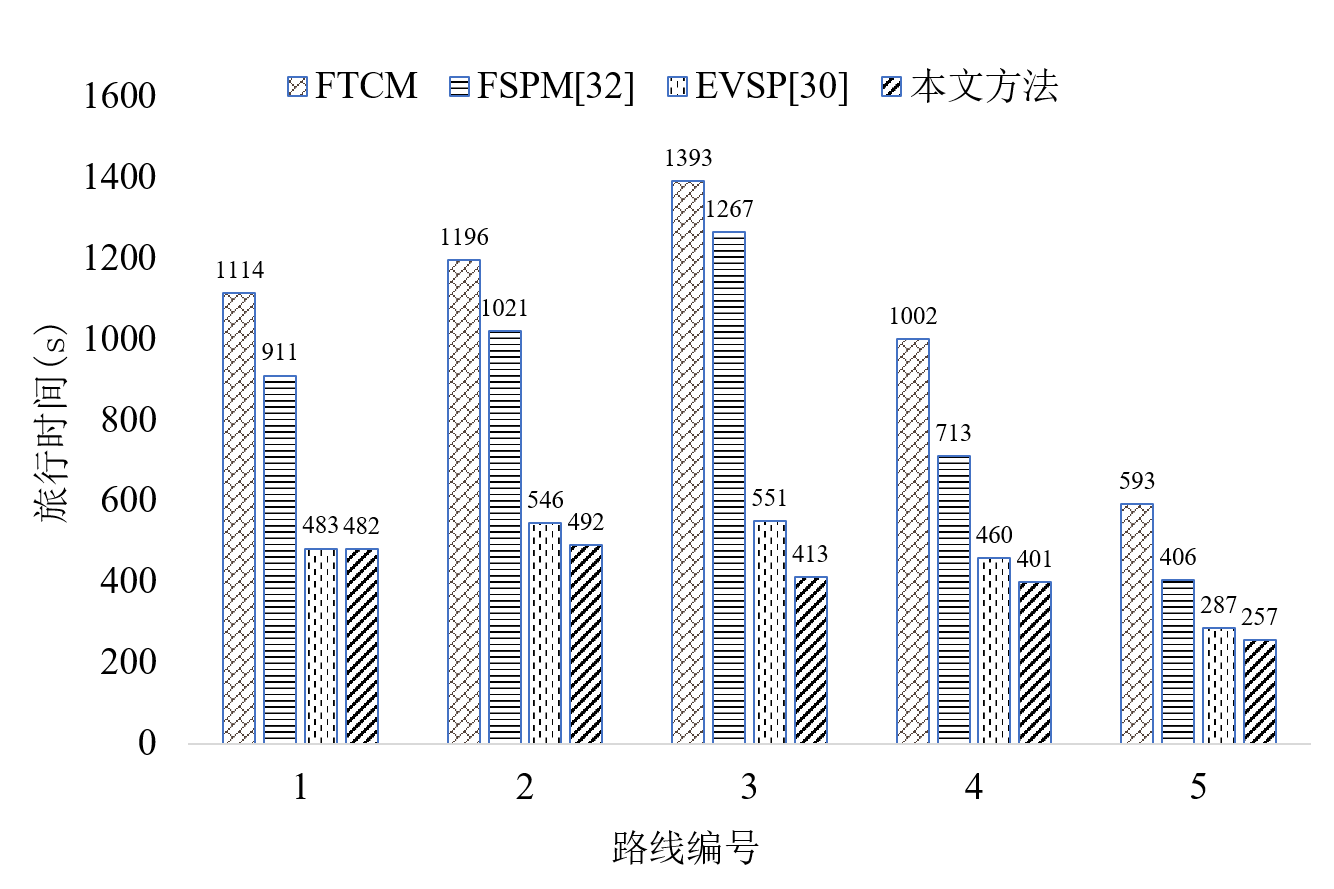
\includegraphics[width=\linewidth]{figures/travel_time2.png}
	\caption{道路比较拥堵时旅行时间比较}
	\label{fig:travel_time_relatively_congestion}
\end{figure}

%图\ref{fig:travel_time_moderate_congestion}表示在道路中度拥堵情况下,5辆应急车辆分别采用FTCM、FSPM、EVSP以及本文方法在路线1至5上的旅行时间。图片表明,本文方法相比于其他三种方法,在道路中度拥堵的情况下仍然具有明显优势。

\begin{figure}[H]
	\centering
	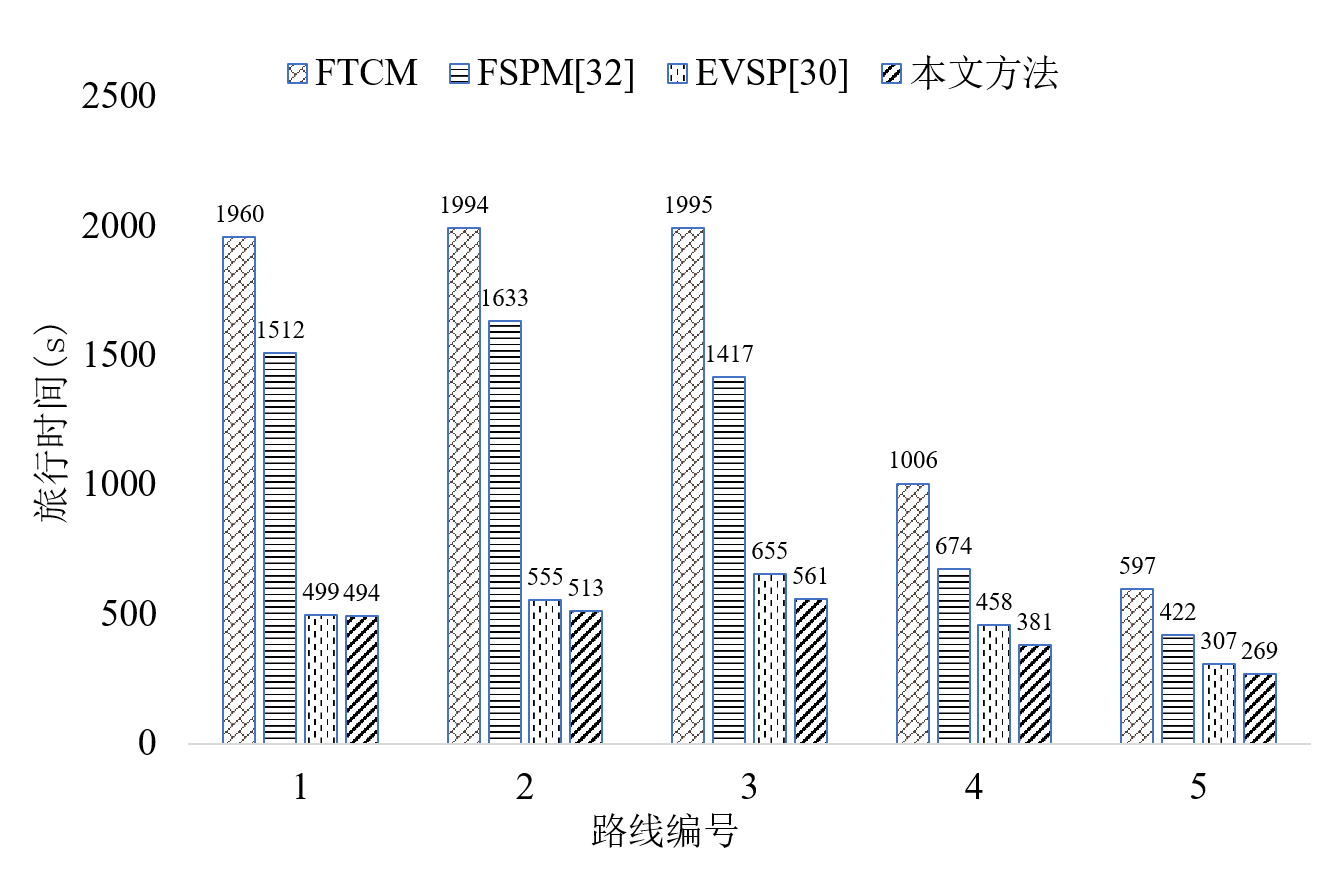
\includegraphics[width=\linewidth]{figures/travel_time3.png}
	\caption{道路中度拥堵时旅行时间比较}
	\label{fig:travel_time_moderate_congestion}
\end{figure}

%图\ref{fig:travel_time_severe_congestion}表示在道路严重拥堵情况下,5辆应急车辆分别采用FTCM、FSPM、EVSP以及本文方法在路线1至5上的旅行时间。图片表明,本文方法相比于其他三种方法,在道路严重拥堵的情况下仍然具有明显优势。

\begin{figure}
	\centering
	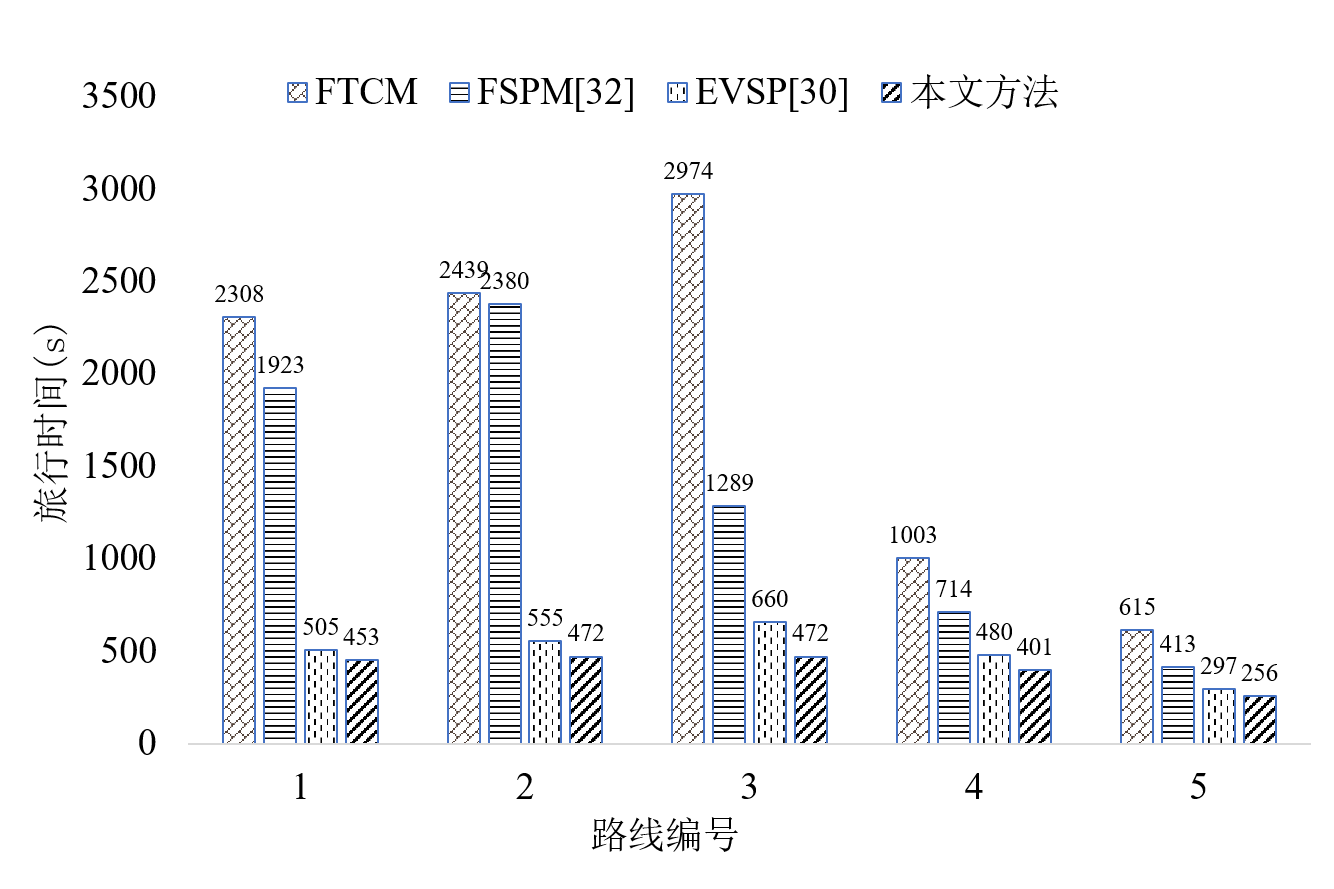
\includegraphics[width=\linewidth]{figures/travel_time4.png}
	\caption{道路严重拥堵时旅行时间比较}
	\label{fig:travel_time_severe_congestion}
\end{figure}

%由此可知,绝大部分情况下本文方法能够有效缩短应急车辆的旅行时间,并且效果非常明显。即使在发生车祸的路段,也能够大幅度缩短应急车辆的旅行时间。

如表\ref{table:travel_time_my_FTCM}所示,在不同交通规模下测试了FTCM与本文方法中应急车辆所需的旅行时间,本文方法旅行时间均值为当前交通规模下,5辆应急车辆在本文方法中旅行时间的平均值,FTCM旅行时间均值为当前交通规模下,5辆应急车辆在FTCM中旅行时间的平均值。实验结果表示,在道路畅通的情况下,本文方法能够优化50.98\%左右。在道路较为拥堵的情况下,本文方法能够优化60.52\%左右。在道路中度拥堵情况下,本文方法能够 优化67.18\%。在道路严重拥堵的情况下,本文方法能够优化72.71\%左右。最终与FTCM相比,本文能够有效缩短应急车辆62.85\%左右的旅行时间。

\begin{table}[H]
	\centering
	\caption{本文方法与FTCM相比旅行时间的优化结果}
	\label{table:travel_time_my_FTCM}
	\begin{tabular}{|c|c|c|c|}
		\hline
		交通规模  & 本文方法旅行时间均值 & FTCM旅行时间均值 & 优化百分比(\%) \\ \hline
		畅通     & 397      & 782     & 50.98  \\ \hline
		比较拥堵 & 409      & 1060    & 60.52  \\ \hline
		中度拥堵 & 444      & 1496    & 67.18  \\ \hline
		严重拥堵 & 411      & 1868    & 72.71  \\ \hline
		  &  &  & 62.85(平均) \\ \hline
	\end{tabular}
\end{table}


如表\ref{table:travel_time_my_FSPM}所示,在不同交通规模下测试了FSPM与本文方法中应急车辆所需的旅行时间,FSPM旅行时间均值为当前交通规模下,5辆应急车辆在使用FSPM时旅行时间的平均值。实验结果表示,在道路畅通的情况下,本文方法相比于FSPM能够优化37.56\%左右。在道路较为拥堵的情况下,本文方法能够优化50.20\%左右。在道路中度拥堵情况下,本文方法能够优化55.21\%。在道路严重拥堵的情况下,本文方法能够优化60.37\%左右。最终与FSPM相比,本文能够有效缩短应急车辆50.84\%左右的旅行时间。

\begin{table}[H]
	\centering
	\caption{本文方法与FSPM相比旅行时间的优化结果}
	\label{table:travel_time_my_FSPM}
	\begin{tabular}{|c|c|c|c|}
		\hline
		交通规模 & 本文方法旅行时间均值 & FSPM旅行时间均值\cite{min} & 优化百分比(\%) \\ \hline
		畅通     & 397 & 610  & 37.56                      \\ \hline
		比较拥堵 & 409 & 880  & 50.20                      \\ \hline
		中度拥堵 & 444 & 1131 & 55.21                      \\ \hline
		严重拥堵 & 411 & 1344 & 60.37                      \\ \hline
		  &  &  & 50.83(平均) \\ \hline
	\end{tabular}
\end{table}

如表\ref{table:travel_time_my_ISPM}所示,在不同交通规模下测试了EVSP与本文方法中应急车辆所需的旅行时间,EVSP旅行时间均值为当前交通规模下,5辆应急车辆在EVSP中旅行时间的平均值。实验结果表示,在道路畅通的情况下,本文方法相比于EVSP能够优化10.59\%左右。在道路较为拥堵的情况下,本文方法能够优化11.68\%左右。在道路中度拥堵情况下,本文方法能够优化10.42\%。在道路严重拥堵的情况下,本文方法能够优化13.80\%左右。最终与EVSP相比,本文能够有效缩短应急车辆16.80\%左右的旅行时间。

\begin{table}[H]
	\centering
	\caption{本文方法与EVSP相比旅行时间的优化结果}
	\label{table:travel_time_my_ISPM}
	\begin{tabular}{|c|c|c|c|}
		\hline
		交通规模	& 本文方法旅行时间均值 & EVSP旅行时间均值\cite{qin_control_2012} & 优化百分比(\%) \\ \hline
		畅通		  & 397     & 423           & 10.59           \\ \hline
		比较拥堵	& 409     & 465           & 11.68           \\ \hline
		中度拥堵	& 444     & 495           & 10.42           \\ \hline
		严重拥堵	& 411     & 499           & 13.80           \\ \hline
		  &  &  & 11.62(平均) \\ \hline
	\end{tabular}
\end{table}

如图\ref{fig:ave_travel_time}所示,将表格中的数据表示在图片当中,把上表的数据用直方图显示出来,横轴是交通规模,纵轴是给定交通规模下五条路线的平均旅行时间。可以看到,在道路畅通、道路较为拥堵、道路中度拥堵以及道路严重拥堵的情况下,本文方法均可有效缩短旅行时间。实验结果表明,与FTCM、FSPM和EVSP相比,本文的策略具有明显的优势。

\begin{figure}[H]
	\centering
	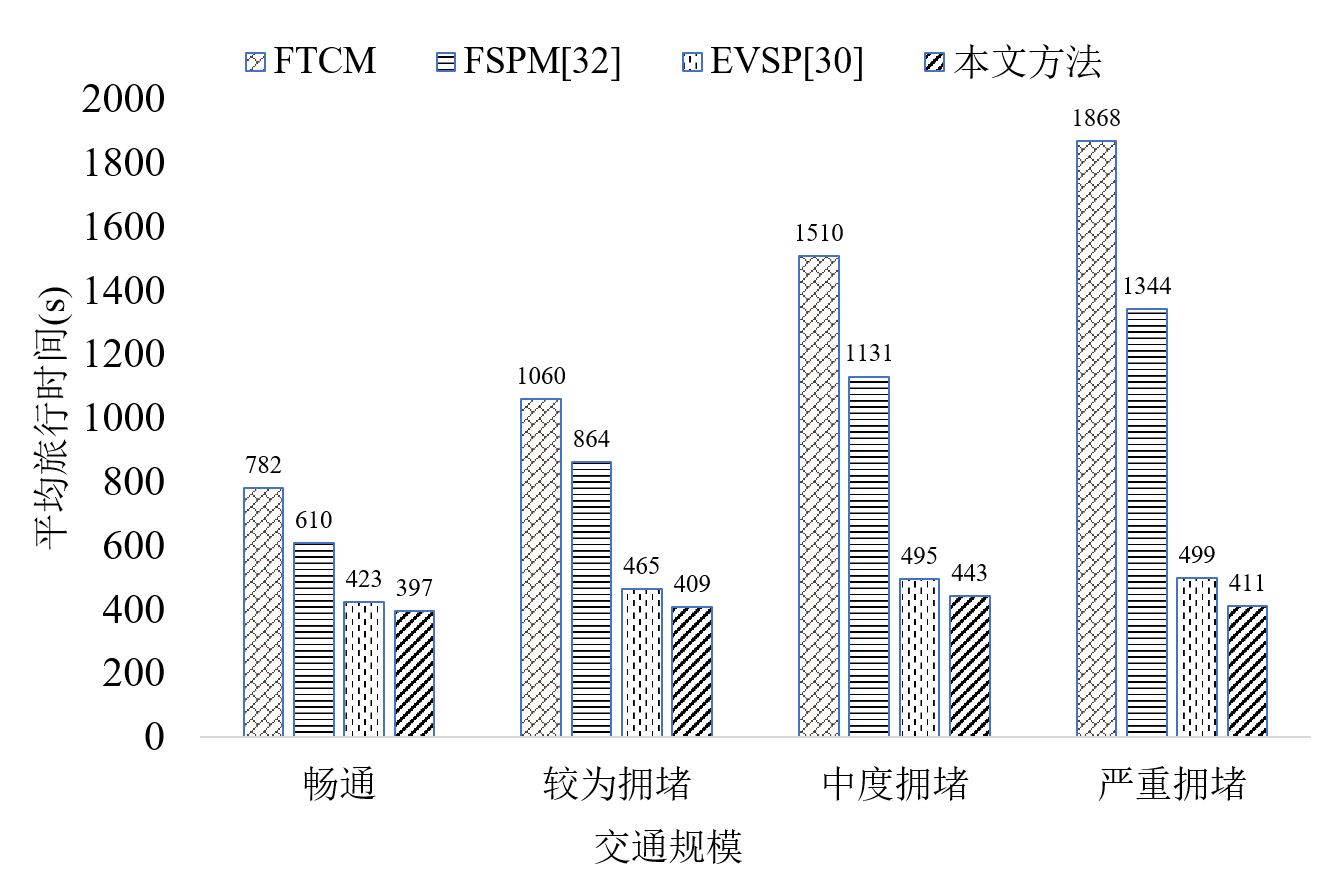
\includegraphics[width=\linewidth]{figures/ave_travel_time.png}
	\caption{不同交通规模下平均旅行时间比较}
	\label{fig:ave_travel_time}
\end{figure}


\subsection{应急车辆优先对路网的影响分析}
为了验证本文方法是否会对整个交通路网造成较大影响,以及测试本文恢复阶段信号控制方案的可用性,测试了应急车辆在不同交通拥堵情况下,整个交通流平均等待时间在本文信号控制方法与固定时长信号控制方法的对比。车辆等待时间表示车速低于或等于0.1m/s的时间,交通流平均等待时间表示交通流中所有车辆等待时间的平均,交通流平均等待时间越大表示道路状况越糟糕,即本文恢复阶段信号控制方案的可用性越低,相反交通流平均等待时间越小表示道路状况越理想,即本文恢复阶段信号控制方案的可用性越高。本文对5辆应急车辆分别在道路畅通、道路较为拥堵、道路中度拥堵以及道路严重拥堵四种交通规模下进行实验,并设置应急响应等级为特别重大(Ⅰ级),再对各交通规模取5次实验的平均值。每一次实验,都记录了从应急车辆出发到应急车辆离开路网后5分钟内整个交通路网中所有车辆的平均等待时间。

由图\ref{fig:waiting_smooth}可知,在道路畅通的情况下,本文方法能够有效缩短整个交通路网的平均等待时间,本文方法不仅对路网没有影响,还意外地起到了疏散交通的作用。由图\ref{fig:waiting_relatively_congestion}可知,在道路比较拥堵的的情况下,应急车辆在路线2、路线4和路线5上的行驶时,使用本文方法能够起到疏散交通的作用,但在路线1和路线3上,本文方法分别延长了平均等待时间7s和4s,这在允许范围内,可视为不对交通造成明显影响。由图\ref{fig:waiting_moderate_congestion}可知,在道路中度拥堵的情况下,应急车辆在路线1、路线2和路线3上的行驶时,使用本文方法能够明显缩短路网的平均等待时间,能够起到疏散交通的作用,在路线4和路线5上表现为不对交通造成明显影响。由图\ref{fig:waiting_severely_congestion}可知,在道路严重拥堵的情况下,应急车辆在路线1和路线2上行驶时,使用本文方法能够明显缩短路网的平均等待时间,能够起到疏散交通的作用。在路线4和路线5上表现为不对交通造成明显影响。在路线3上表现为影响了整个交通,这是由于在实验过程中,应急车辆在行驶过程中遇到了车祸,导致整个交通出现了瘫痪。

\begin{figure}[H]
	\centering
	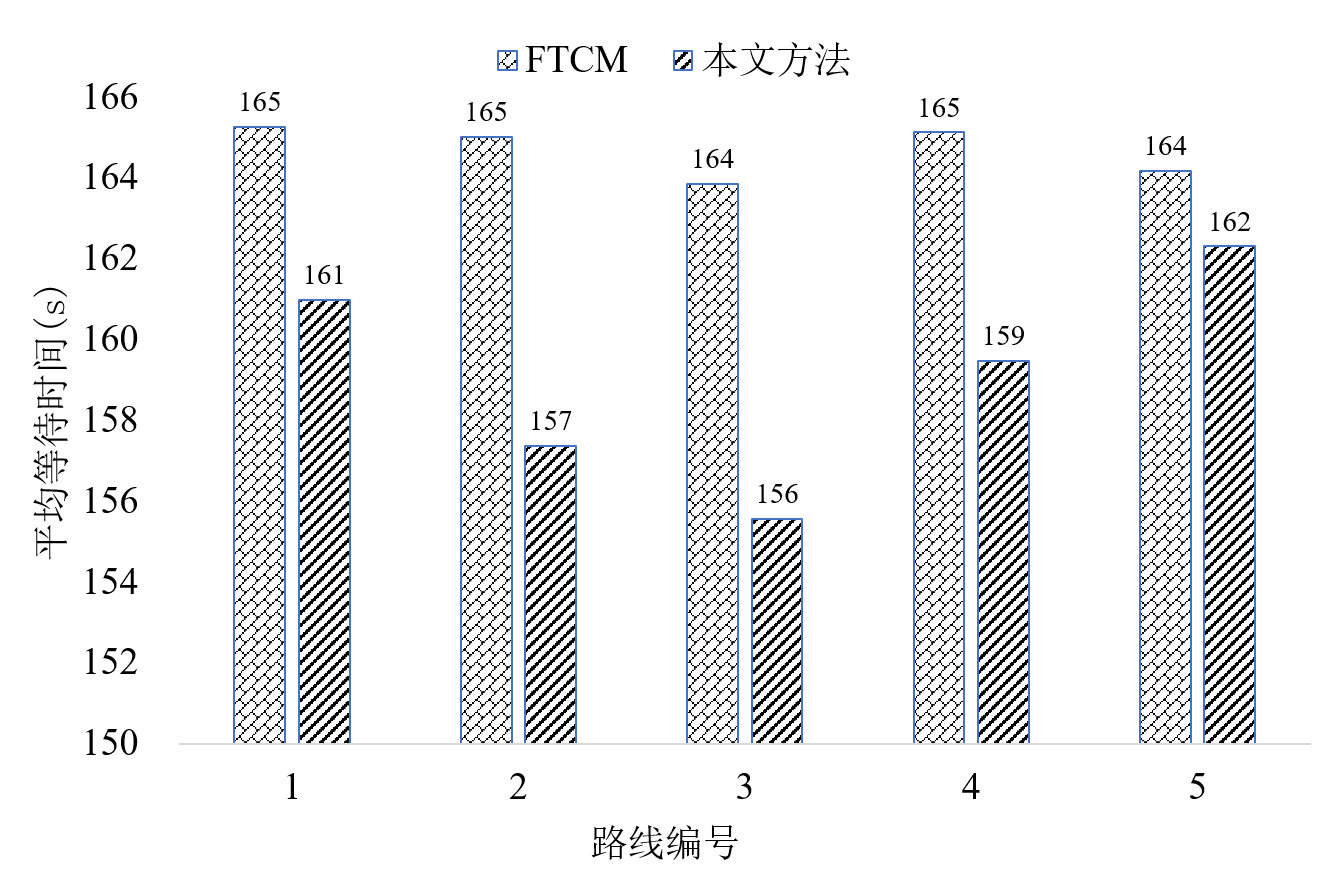
\includegraphics[width=\linewidth]{figures/awt1.png}
	\caption{道路畅通时平均等待时间比较}
	\label{fig:waiting_smooth}
\end{figure}

%由图\ref{fig:waiting_relatively_congestion}可知,在道路比较拥堵的的情况下,应急车辆在路线2、路线4和路线5上的行驶时,使用本文方法能够起到疏散交通的作用,但在路线1和路线3上,本文方法分别延长了平均等待时间7s和4s,这在允许范围内,可视为不对交通造成明显影响。

%由图\ref{fig:waiting_moderate_congestion}可知,在道路中度拥堵的情况下,应急车辆在路线1、路线2和路线3上的行驶时,使用本文方法能够明显缩短路网的平均等待时间,能够起到疏散交通的作用,在路线4和路线5上表现为不对交通造成明显影响。

%由图\ref{fig:waiting_severely_congestion}可知,在道路严重拥堵的情况下,应急车辆在路线1和路线2上行驶时,使用本文方法能够明显缩短路网的平均等待时间,能够起到疏散交通的作用。在路线4和路线5上表现为不对交通造成明显影响。在路线3上表现为影响了整个交通,这是由于在实验过程中,应急车辆在行驶过程中遇到了车祸,导致整个交通出现了瘫痪。

\begin{figure}[H]
	\centering
	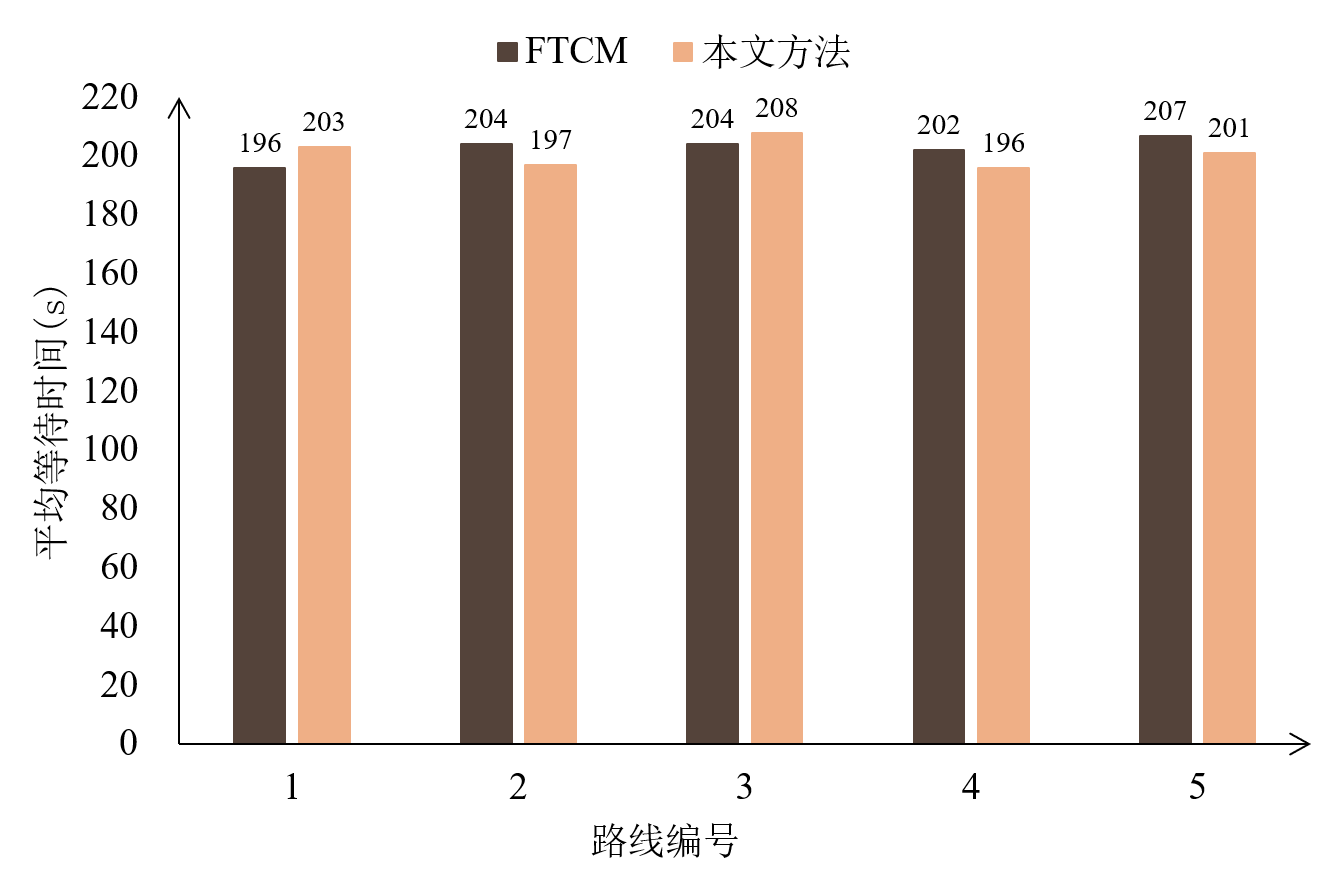
\includegraphics[width=\linewidth]{figures/awt2.png}
	\caption{道路比较拥堵时平均等待时间比较}
	\label{fig:waiting_relatively_congestion}
\end{figure}
\begin{figure}[H]
	\centering
	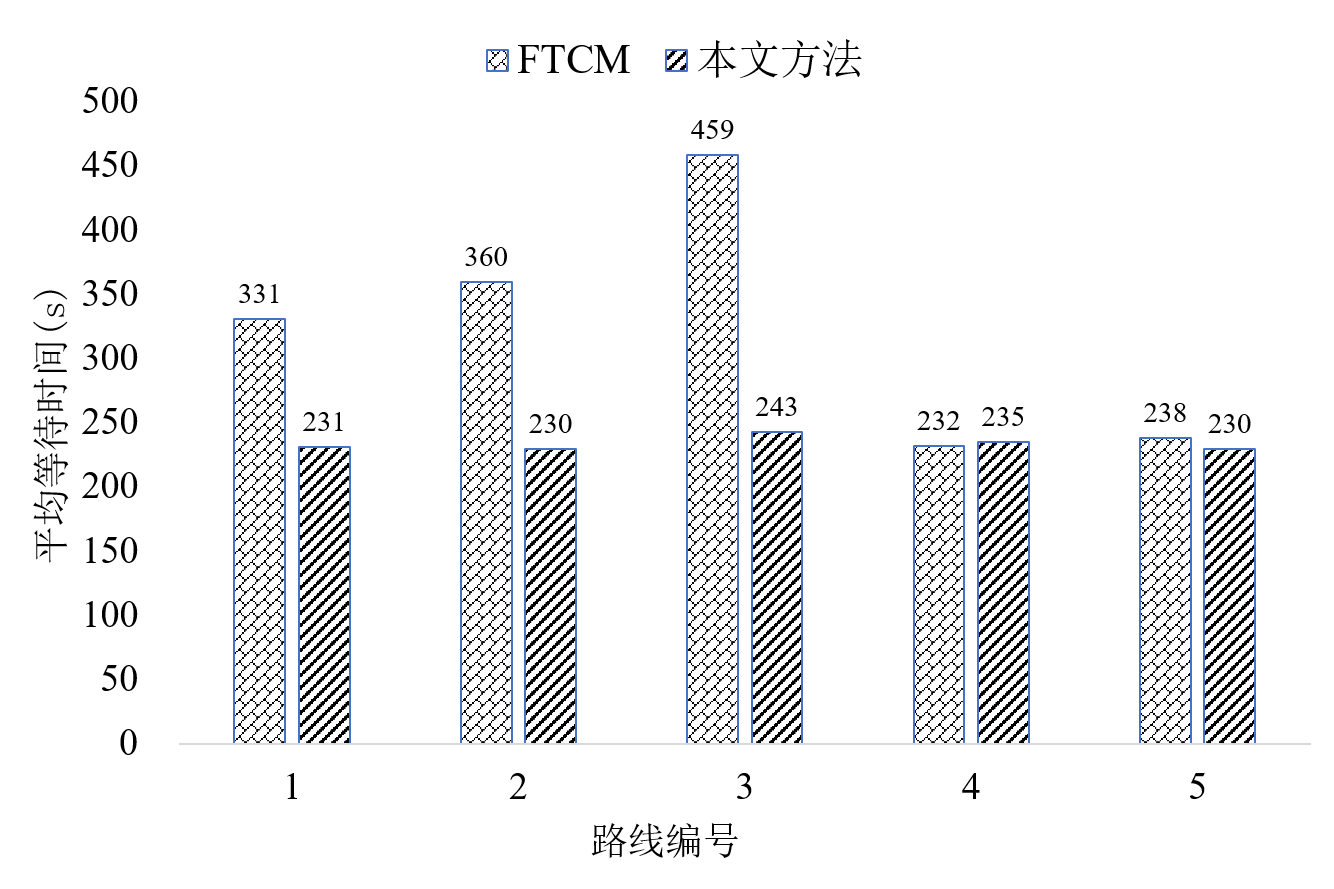
\includegraphics[width=\linewidth]{figures/awt3.png}
	\caption{道路中度拥堵时平均等待时间比较}
	\label{fig:waiting_moderate_congestion}
\end{figure}
\begin{figure}[H]
	\centering
	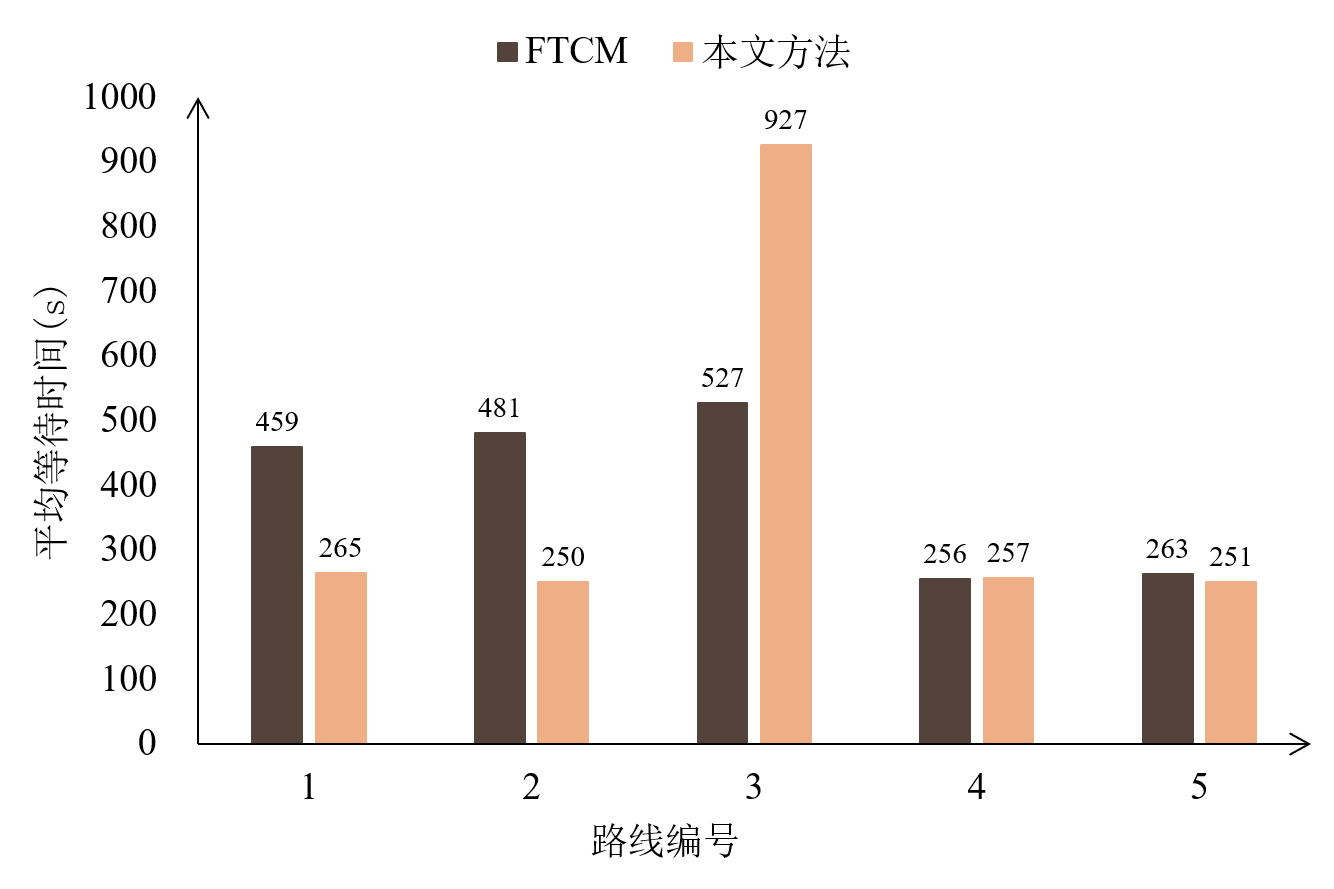
\includegraphics[width=\linewidth]{figures/awt4.png}
	\caption{道路严重拥堵时平均等待时间比较}
	\label{fig:waiting_severely_congestion}
\end{figure}

图\ref{fig:awt_conclude}中横坐标表示在道路畅通、道路比较拥堵、道路中度拥堵和道路严重拥堵四种交通规模下,纵坐标表示路网平均等待时间的平均。从图中可以看出,由于恢复交通流阶段信号控制方法,本文信号控制方案能够有效地降低应急车辆优先通行对整个交通流造成的影响,并且还在一定程度上对交通流起到了疏散的作用。

\begin{figure}[H]
	\centering
	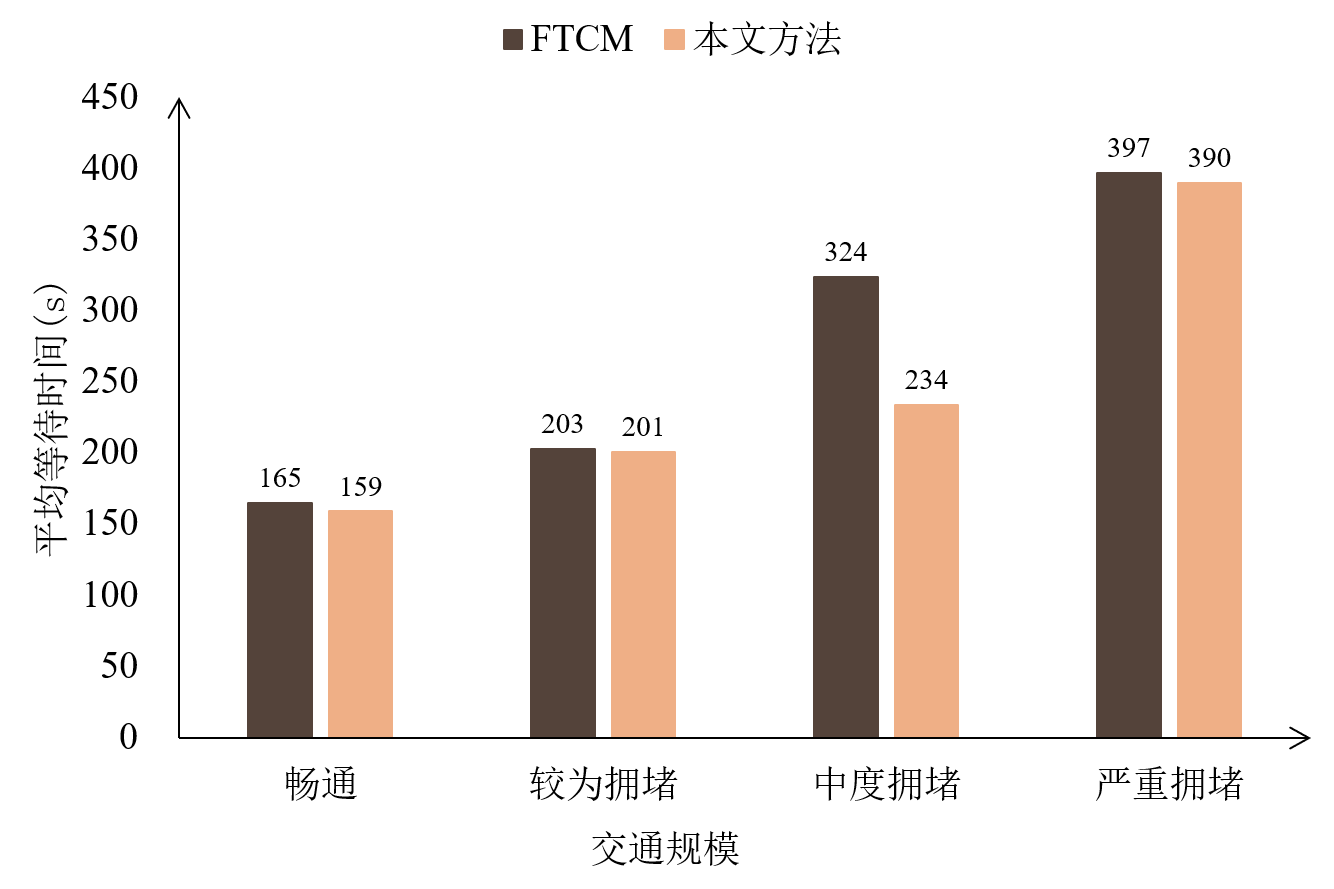
\includegraphics[width=\linewidth]{figures/awt_conclude.png}
	\caption{不同交通规模下平均等待时间的比较}
	\label{fig:awt_conclude}
\end{figure}

\section{实验分析与总结}
本文提出了一种新颖的面向应急车辆优先通行的交通信号灯智能控制方法,该策略分为三个步骤:(1)按需降低道路饱和度及普通车辆让行;(2)信号抢占方法;(3)恢复交通流。第一步根据应急响应等级、路段拥堵等级以及时间紧迫等级得出降低道路饱和度的迫切程度值,交叉路口智能体控制交通灯延长应急车辆入口车道方向的绿灯时间,从而降低该方向的道路饱和度。从实验结果可以看到,应急车辆的速度方差与不采取本文方法的固定时长信号控制方法相比,有很明显的下降趋势,因此本文方法能够有效地降低应急车辆前进方向的道路饱和度;第二步分为信号抢占,当非侵入式信号抢占方法无法得出可行的信号相位配置方案时,采取侵入式信号抢占方法,以保证应急车辆不在交叉路口停车,一路畅通。从实验结果可以看到,本文方法能够明显缩短应急车辆的旅行时间,因此本文的信号抢占方法行之有效,且具有超前性;第三步恢复交通流,由于应急车辆的优先通行,可能会对整个路网造成负面影响,因此采用本文的信号恢复策略进行了实验,实验结果表明,采取恢复交通流方法之后,能够有效地降低应急车辆优先对整个路网造成的负面影响,在部分交通情况下,甚至能够舒缓交通,对整个路网交通流有利。
\section{本章小结}
本章对本文提出一种面向应急车辆优先通行的交通信号灯智能控制方法进行了实验评估与分析。首先探讨了实验的目的,然后针对本文方法进行了实验设计,并阐述了实验环境与参数设置,再对应急车辆的速度平稳性、旅行时间以及整个交通路网的平均等待时间进行了分析,最后对实验进行了分析与总结。
